\documentclass[a4paper]{book}
\usepackage{makeidx}
\usepackage{natbib}
\usepackage{graphicx}
\usepackage{multicol}
\usepackage{float}
\usepackage{listings}
\usepackage{color}
\usepackage{ifthen}
\usepackage[table]{xcolor}
\usepackage{textcomp}
\usepackage{alltt}
\usepackage{ifpdf}
\ifpdf
\usepackage[pdftex,
            pagebackref=true,
            colorlinks=true,
            linkcolor=blue,
            unicode
           ]{hyperref}
\else
\usepackage[ps2pdf,
            pagebackref=true,
            colorlinks=true,
            linkcolor=blue,
            unicode
           ]{hyperref}
\usepackage{pspicture}
\fi
\usepackage[utf8]{inputenc}
\usepackage[ngerman]{babel}

\usepackage{mathptmx}
\usepackage[scaled=.90]{helvet}
\usepackage{courier}
\usepackage{sectsty}
\usepackage[titles]{tocloft}
\usepackage{doxygen}
\lstset{language=C++,inputencoding=utf8,basicstyle=\footnotesize,breaklines=true,breakatwhitespace=true,tabsize=8,numbers=left }
\makeindex
\setcounter{tocdepth}{3}
\renewcommand{\footrulewidth}{0.4pt}
\renewcommand{\familydefault}{\sfdefault}
\hfuzz=15pt
\setlength{\emergencystretch}{15pt}
\hbadness=750
\tolerance=750
\begin{document}
\hypersetup{pageanchor=false,citecolor=blue}
\begin{titlepage}
\vspace*{7cm}
\begin{center}
{\Large \-Lo\-Co-\/\-Cro\-Co\-Wheele }\\
\vspace*{1cm}
{\large \-Erzeugt von Doxygen 1.7.6.1}\\
\vspace*{0.5cm}
{\small Mon Nov 12 2012 21:43:36}\\
\end{center}
\end{titlepage}
\clearemptydoublepage
\pagenumbering{roman}
\tableofcontents
\clearemptydoublepage
\pagenumbering{arabic}
\hypersetup{pageanchor=true,citecolor=blue}
\chapter{\-Klassen-\/\-Verzeichnis}
\section{\-Klassenhierarchie}
\-Die \-Liste der \-Ableitungen ist -\/mit \-Einschränkungen-\/ alphabetisch sortiert\-:\begin{DoxyCompactList}
\item \contentsline{section}{\-C\-Actor}{\pageref{class_c_actor}}{}
\begin{DoxyCompactList}
\item \contentsline{section}{\-C\-Motor}{\pageref{class_c_motor}}{}
\item \contentsline{section}{\-C\-P\-W\-M\-Driver}{\pageref{class_c_p_w_m_driver}}{}
\end{DoxyCompactList}
\item \contentsline{section}{\-C\-I2\-C}{\pageref{class_c_i2_c}}{}
\item \contentsline{section}{\-C\-Kalman\-Filter}{\pageref{class_c_kalman_filter}}{}
\item \contentsline{section}{\-C\-Logger}{\pageref{class_c_logger}}{}
\item \contentsline{section}{\-C\-P\-I\-D\-Regler}{\pageref{class_c_p_i_d_regler}}{}
\item \contentsline{section}{\-C\-P\-W\-M}{\pageref{class_c_p_w_m}}{}
\item \contentsline{section}{\-C\-Sensor}{\pageref{class_c_sensor}}{}
\begin{DoxyCompactList}
\item \contentsline{section}{\-C\-B\-M\-A180}{\pageref{class_c_b_m_a180}}{}
\item \contentsline{section}{\-C\-I\-T\-G3200}{\pageref{class_c_i_t_g3200}}{}
\item \contentsline{section}{\-C\-L\-S\-M303\-D\-L\-H}{\pageref{class_c_l_s_m303_d_l_h}}{}
\item \contentsline{section}{\-C\-R\-P\-Meter}{\pageref{class_c_r_p_meter}}{}
\end{DoxyCompactList}
\item \contentsline{section}{\-C\-Server}{\pageref{class_c_server}}{}
\item \contentsline{section}{\-C\-Vector}{\pageref{class_c_vector}}{}
\end{DoxyCompactList}

\chapter{\-Klassen-\/\-Verzeichnis}
\section{\-Auflistung der \-Klassen}
\-Hier folgt die \-Aufzählung aller \-Klassen, \-Strukturen, \-Varianten und \-Schnittstellen mit einer \-Kurzbeschreibung\-:\begin{DoxyCompactList}
\item\contentsline{section}{\hyperlink{class_c_actor}{\-C\-Actor} }{\pageref{class_c_actor}}{}
\item\contentsline{section}{\hyperlink{class_c_b_m_a180}{\-C\-B\-M\-A180} }{\pageref{class_c_b_m_a180}}{}
\item\contentsline{section}{\hyperlink{class_c_i2_c}{\-C\-I2\-C} }{\pageref{class_c_i2_c}}{}
\item\contentsline{section}{\hyperlink{class_c_i_t_g3200}{\-C\-I\-T\-G3200} }{\pageref{class_c_i_t_g3200}}{}
\item\contentsline{section}{\hyperlink{class_c_kalman_filter}{\-C\-Kalman\-Filter} }{\pageref{class_c_kalman_filter}}{}
\item\contentsline{section}{\hyperlink{class_c_logger}{\-C\-Logger} }{\pageref{class_c_logger}}{}
\item\contentsline{section}{\hyperlink{class_c_l_s_m303_d_l_h}{\-C\-L\-S\-M303\-D\-L\-H} }{\pageref{class_c_l_s_m303_d_l_h}}{}
\item\contentsline{section}{\hyperlink{class_c_motor}{\-C\-Motor} }{\pageref{class_c_motor}}{}
\item\contentsline{section}{\hyperlink{class_c_p_i_d_regler}{\-C\-P\-I\-D\-Regler} }{\pageref{class_c_p_i_d_regler}}{}
\item\contentsline{section}{\hyperlink{class_c_p_w_m}{\-C\-P\-W\-M} }{\pageref{class_c_p_w_m}}{}
\item\contentsline{section}{\hyperlink{class_c_p_w_m_driver}{\-C\-P\-W\-M\-Driver} }{\pageref{class_c_p_w_m_driver}}{}
\item\contentsline{section}{\hyperlink{class_c_r_p_meter}{\-C\-R\-P\-Meter} }{\pageref{class_c_r_p_meter}}{}
\item\contentsline{section}{\hyperlink{class_c_sensor}{\-C\-Sensor} }{\pageref{class_c_sensor}}{}
\item\contentsline{section}{\hyperlink{class_c_server}{\-C\-Server} }{\pageref{class_c_server}}{}
\item\contentsline{section}{\hyperlink{class_c_vector}{\-C\-Vector} }{\pageref{class_c_vector}}{}
\end{DoxyCompactList}

\chapter{\-Klassen-\/\-Dokumentation}
\hypertarget{class_c_actor}{\section{\-C\-Actor \-Klassenreferenz}
\label{class_c_actor}\index{\-C\-Actor@{\-C\-Actor}}
}
\-Klassendiagramm für \-C\-Actor\-:\begin{figure}[H]
\begin{center}
\leavevmode
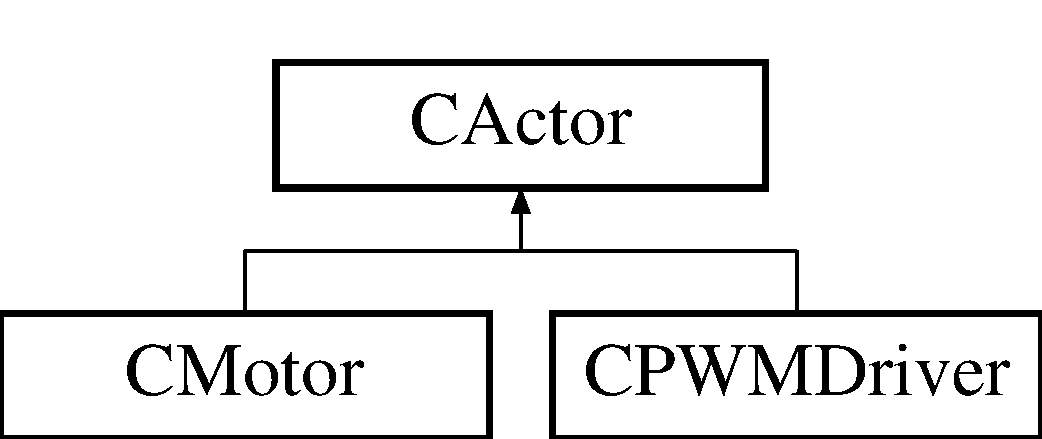
\includegraphics[height=2.000000cm]{class_c_actor}
\end{center}
\end{figure}
\subsection*{Öffentliche \-Methoden}
\begin{DoxyCompactItemize}
\item 
\hyperlink{class_c_actor_a22436a9e69474d47f31ac81fa192ba4b}{\-C\-Actor} ()
\item 
virtual \hyperlink{class_c_actor_a1ff541702c90c8c5ec57aff57568ef04}{$\sim$\-C\-Actor} ()
\item 
virtual bool \hyperlink{class_c_actor_a8a04a31e44aaa861d97bdbeb7ae1a570}{set\-Value} (float i\-Value, uint8\-\_\-t i\-Channle)=0
\end{DoxyCompactItemize}


\subsection{\-Beschreibung der \-Konstruktoren und \-Destruktoren}
\hypertarget{class_c_actor_a22436a9e69474d47f31ac81fa192ba4b}{\index{\-C\-Actor@{\-C\-Actor}!\-C\-Actor@{\-C\-Actor}}
\index{\-C\-Actor@{\-C\-Actor}!CActor@{\-C\-Actor}}
\subsubsection[{\-C\-Actor}]{\setlength{\rightskip}{0pt plus 5cm}{\bf \-C\-Actor\-::\-C\-Actor} (
\begin{DoxyParamCaption}
{}
\end{DoxyParamCaption}
)}}\label{class_c_actor_a22436a9e69474d47f31ac81fa192ba4b}
\-Erzeugt ein \-Objekt der \-Klasse \hyperlink{class_c_actor}{\-C\-Actor}. \hypertarget{class_c_actor_a1ff541702c90c8c5ec57aff57568ef04}{\index{\-C\-Actor@{\-C\-Actor}!$\sim$\-C\-Actor@{$\sim$\-C\-Actor}}
\index{$\sim$\-C\-Actor@{$\sim$\-C\-Actor}!CActor@{\-C\-Actor}}
\subsubsection[{$\sim$\-C\-Actor}]{\setlength{\rightskip}{0pt plus 5cm}virtual {\bf \-C\-Actor\-::$\sim$\-C\-Actor} (
\begin{DoxyParamCaption}
{}
\end{DoxyParamCaption}
)\hspace{0.3cm}{\ttfamily  \mbox{[}virtual\mbox{]}}}}\label{class_c_actor_a1ff541702c90c8c5ec57aff57568ef04}
\-Löscht ein \-Objekt der \-Klasse \hyperlink{class_c_actor}{\-C\-Actor}. 

\subsection{\-Dokumentation der \-Elementfunktionen}
\hypertarget{class_c_actor_a8a04a31e44aaa861d97bdbeb7ae1a570}{\index{\-C\-Actor@{\-C\-Actor}!set\-Value@{set\-Value}}
\index{set\-Value@{set\-Value}!CActor@{\-C\-Actor}}
\subsubsection[{set\-Value}]{\setlength{\rightskip}{0pt plus 5cm}virtual bool {\bf \-C\-Actor\-::set\-Value} (
\begin{DoxyParamCaption}
\item[{float}]{i\-Value, }
\item[{uint8\-\_\-t}]{i\-Channle}
\end{DoxyParamCaption}
)\hspace{0.3cm}{\ttfamily  \mbox{[}pure virtual\mbox{]}}}}\label{class_c_actor_a8a04a31e44aaa861d97bdbeb7ae1a570}
\-Gibt den \-Wert i\-Value an den \-Datenkanal i\-Channel weiter. 
\begin{DoxyParams}[1]{\-Parameter}
\mbox{\tt in}  & {\em i\-Value} & \-Wert der übergeben werden soll. \\
\hline
\mbox{\tt in}  & {\em i\-Channle} & \-Datenkanal an dem der \-Wert i\-Value übergeben werden soll. \\
\hline
\end{DoxyParams}
\begin{DoxyReturn}{\-Rückgabe}
\-Gibt zurück ob der \-Wert i\-Value in den \-Datenkanal i\-Channle übergeben werden konnte, bzw. ob es den aufgerufenen \-Datenkanal gibt. 
\end{DoxyReturn}


\-Implementiert in \hyperlink{class_c_p_w_m_driver_a91a128c891a11d64ba7a8d1486e77fab}{\-C\-P\-W\-M\-Driver} und \hyperlink{class_c_motor_a83fa60cbf910c7386fb45db8ea875de1}{\-C\-Motor}.



\-Die \-Dokumentation für diese \-Klasse wurde erzeugt aufgrund der \-Datei\-:\begin{DoxyCompactItemize}
\item 
include/\-C\-Actor.\-h\end{DoxyCompactItemize}

\hypertarget{class_c_b_m_a180}{\section{\-C\-B\-M\-A180 \-Klassenreferenz}
\label{class_c_b_m_a180}\index{\-C\-B\-M\-A180@{\-C\-B\-M\-A180}}
}
\-Klassendiagramm für \-C\-B\-M\-A180\-:\begin{figure}[H]
\begin{center}
\leavevmode
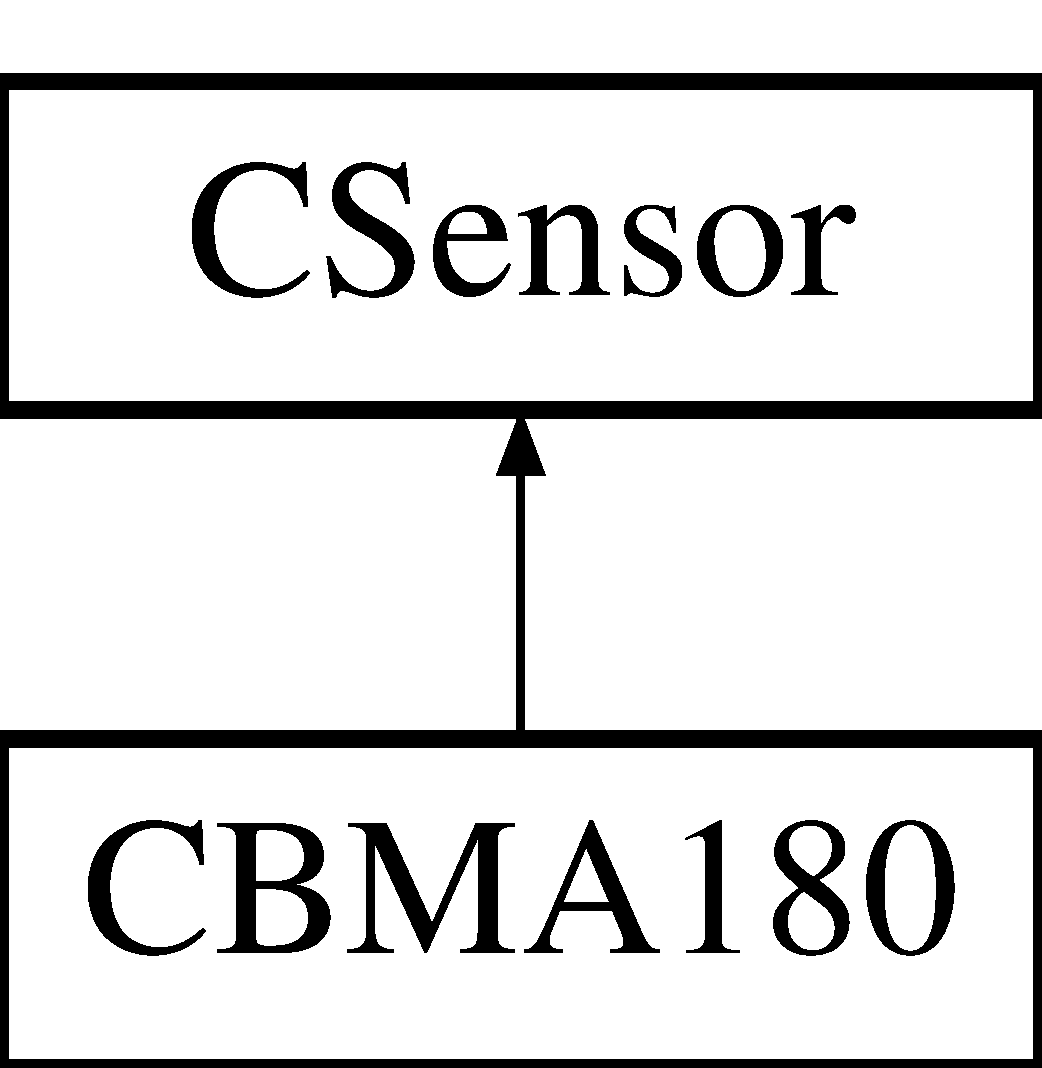
\includegraphics[height=2.000000cm]{class_c_b_m_a180}
\end{center}
\end{figure}
\subsection*{Öffentliche \-Methoden}
\begin{DoxyCompactItemize}
\item 
\hyperlink{class_c_b_m_a180_a4f07fb4e031d55899dda017623301cfd}{\-C\-B\-M\-A180} (\hyperlink{class_c_i2_c}{\-C\-I2\-C} $\ast$p\-I2\-C, uint8\-\_\-t i\-Address)
\item 
virtual \hyperlink{class_c_b_m_a180_a4ee1ab160be5e9839ec62045283d9b63}{$\sim$\-C\-B\-M\-A180} ()
\item 
uint16\-\_\-t \hyperlink{class_c_b_m_a180_af45e95b6cef3448e758cf9c407b219cf}{get\-Acc\-X\-Raw} ()
\item 
uint16\-\_\-t \hyperlink{class_c_b_m_a180_af21a35191db52dee7c271d44da42bd2f}{get\-Acc\-Y\-Raw} ()
\item 
uint16\-\_\-t \hyperlink{class_c_b_m_a180_a5f4f8579e3eb267ad3b1ac828a99ece8}{get\-Acc\-Z\-Raw} ()
\item 
int16\-\_\-t \hyperlink{class_c_b_m_a180_aafcebbbc6fa319c83467ea2918360802}{get\-Acc\-X\-Signed\-Raw} ()
\item 
int16\-\_\-t \hyperlink{class_c_b_m_a180_a05accbd8a3ddf864c41bc1ef9cfb1590}{get\-Acc\-Y\-Signed\-Raw} ()
\item 
int16\-\_\-t \hyperlink{class_c_b_m_a180_af2f8ed8bdbbaa33ea051de0b4690f49b}{get\-Acc\-Z\-Signed\-Raw} ()
\item 
float \hyperlink{class_c_b_m_a180_a7e1b7e8a3dc7e35d660285648bbf2cd8}{get\-Acc\-X} ()
\item 
float \hyperlink{class_c_b_m_a180_a15562c533c3e3ecf09ee6434ad9ba349}{get\-Acc\-Y} ()
\item 
float \hyperlink{class_c_b_m_a180_a13878be864d0c1c86fb5da9a7bed1bef}{get\-Acc\-Z} ()
\item 
float \hyperlink{class_c_b_m_a180_a1479e687581a037339e5db0a26183069}{get\-Acc\-Alpha} ()
\item 
float \hyperlink{class_c_b_m_a180_a1eb83ff966920cba25c3506f90cc36f1}{get\-Acc\-Beta} ()
\item 
float \hyperlink{class_c_b_m_a180_aaef74ead21abf6fc87647ad5f63c5a03}{get\-Acc\-Gamma} ()
\item 
\hyperlink{class_c_vector}{\-C\-Vector} \hyperlink{class_c_b_m_a180_ac9344e2d63aee2f5a1ad23156e2bbfc0}{get\-Vector} ()
\item 
uint16\-\_\-t \hyperlink{class_c_b_m_a180_a989e2bdc2ac1fc5e228d469c7ed99187}{get\-Acc\-X\-Raw\-Per\-I2\-C} ()
\item 
uint16\-\_\-t \hyperlink{class_c_b_m_a180_a2b37888a1df1fd1d0c17c95bb6c7e15a}{get\-Acc\-Y\-Raw\-Per\-I2\-C} ()
\item 
uint16\-\_\-t \hyperlink{class_c_b_m_a180_accd1c61c0323e5acbd47cd1b1176084f}{get\-Acc\-Z\-Raw\-Per\-I2\-C} ()
\item 
int16\-\_\-t \hyperlink{class_c_b_m_a180_aca9a02a8a24b408f1a27de0f6303491f}{get\-Acc\-X\-Signed\-Raw\-Per\-I2\-C} ()
\item 
\hypertarget{class_c_b_m_a180_a76d299e0ede75e23c7c27b15391ffc2a}{int16\-\_\-t {\bfseries get\-Acc\-Y\-Signed\-Raw\-Per\-I2\-C} ()}\label{class_c_b_m_a180_a76d299e0ede75e23c7c27b15391ffc2a}

\item 
\hypertarget{class_c_b_m_a180_a70079e27326d0123a0b79ae2c2e1eb65}{int16\-\_\-t {\bfseries get\-Acc\-Z\-Signed\-Raw\-Per\-I2\-C} ()}\label{class_c_b_m_a180_a70079e27326d0123a0b79ae2c2e1eb65}

\item 
\hypertarget{class_c_b_m_a180_ab11c44f987669179c5172b1b77f9b633}{float {\bfseries get\-Acc\-X\-Per\-I2\-C} ()}\label{class_c_b_m_a180_ab11c44f987669179c5172b1b77f9b633}

\item 
\hypertarget{class_c_b_m_a180_ad60528a9b4b1c1ec6cad32b734930476}{float {\bfseries get\-Acc\-Y\-Per\-I2\-C} ()}\label{class_c_b_m_a180_ad60528a9b4b1c1ec6cad32b734930476}

\item 
\hypertarget{class_c_b_m_a180_a6d43bec30f5b932cc5615865af86a66a}{float {\bfseries get\-Acc\-Z\-Per\-I2\-C} ()}\label{class_c_b_m_a180_a6d43bec30f5b932cc5615865af86a66a}

\item 
\hypertarget{class_c_b_m_a180_a03c043a3e8ebb7cc7fac3c5153ba356d}{float {\bfseries get\-Acc\-Alpha\-Per\-I2\-C} ()}\label{class_c_b_m_a180_a03c043a3e8ebb7cc7fac3c5153ba356d}

\item 
\hypertarget{class_c_b_m_a180_afbc6e53796fead89dd732dd18f603d06}{float {\bfseries get\-Acc\-Beta\-Per\-I2\-C} ()}\label{class_c_b_m_a180_afbc6e53796fead89dd732dd18f603d06}

\item 
\hypertarget{class_c_b_m_a180_a8d1de9aea21c4ca82400eb5957e52166}{float {\bfseries get\-Acc\-Gamma\-Per\-I2\-C} ()}\label{class_c_b_m_a180_a8d1de9aea21c4ca82400eb5957e52166}

\item 
\hypertarget{class_c_b_m_a180_ab335f152d838dda55ac631835bc72702}{\hyperlink{class_c_vector}{\-C\-Vector} {\bfseries get\-Vector\-Per\-I2\-C} ()}\label{class_c_b_m_a180_ab335f152d838dda55ac631835bc72702}

\item 
\hypertarget{class_c_b_m_a180_ad026d7a4be6c394c5826a667fc2803c8}{void {\bfseries start} ()}\label{class_c_b_m_a180_ad026d7a4be6c394c5826a667fc2803c8}

\item 
\hypertarget{class_c_b_m_a180_a9c54282ad9d0ea67093ae901f4205869}{void {\bfseries stop} ()}\label{class_c_b_m_a180_a9c54282ad9d0ea67093ae901f4205869}

\item 
\hypertarget{class_c_b_m_a180_a76999767859139f406b78aca9aacb202}{void {\bfseries kill} ()}\label{class_c_b_m_a180_a76999767859139f406b78aca9aacb202}

\item 
\hypertarget{class_c_b_m_a180_ad3ee3468195d3473ffbc3a9cbd8e6e5f}{void {\bfseries run} ()}\label{class_c_b_m_a180_ad3ee3468195d3473ffbc3a9cbd8e6e5f}

\item 
virtual bool \hyperlink{class_c_b_m_a180_a3b4fca3c7e96f59da8f53c5a795cbbcb}{get\-Value} (float \&i\-Value, uint8\-\_\-t i\-Channle)
\end{DoxyCompactItemize}


\subsection{\-Beschreibung der \-Konstruktoren und \-Destruktoren}
\hypertarget{class_c_b_m_a180_a4f07fb4e031d55899dda017623301cfd}{\index{\-C\-B\-M\-A180@{\-C\-B\-M\-A180}!\-C\-B\-M\-A180@{\-C\-B\-M\-A180}}
\index{\-C\-B\-M\-A180@{\-C\-B\-M\-A180}!CBMA180@{\-C\-B\-M\-A180}}
\subsubsection[{\-C\-B\-M\-A180}]{\setlength{\rightskip}{0pt plus 5cm}{\bf \-C\-B\-M\-A180\-::\-C\-B\-M\-A180} (
\begin{DoxyParamCaption}
\item[{{\bf \-C\-I2\-C} $\ast$}]{p\-I2\-C, }
\item[{uint8\-\_\-t}]{i\-Address}
\end{DoxyParamCaption}
)}}\label{class_c_b_m_a180_a4f07fb4e031d55899dda017623301cfd}
\-Erzeugt ein \-Objekt der \-Klasse \hyperlink{class_c_b_m_a180}{\-C\-B\-M\-A180}. \-Der \-Konstruktor erwartet als \-Parameter die i2c \-Adresse des \-Sensors und ein i2c \-Bus \-Objekt über den der \-Sensor ansgeschlossen ist. 
\begin{DoxyParams}[1]{\-Parameter}
\mbox{\tt in}  & {\em p\-I2\-C} & \-Der i2c \-Bus über dem der \-Sensor angeschlossen ist. \\
\hline
\mbox{\tt in}  & {\em i\-Address} & \-Die \-Adresse des \-Sensors auf dem i2c \-Bus. \\
\hline
\end{DoxyParams}
\hypertarget{class_c_b_m_a180_a4ee1ab160be5e9839ec62045283d9b63}{\index{\-C\-B\-M\-A180@{\-C\-B\-M\-A180}!$\sim$\-C\-B\-M\-A180@{$\sim$\-C\-B\-M\-A180}}
\index{$\sim$\-C\-B\-M\-A180@{$\sim$\-C\-B\-M\-A180}!CBMA180@{\-C\-B\-M\-A180}}
\subsubsection[{$\sim$\-C\-B\-M\-A180}]{\setlength{\rightskip}{0pt plus 5cm}virtual {\bf \-C\-B\-M\-A180\-::$\sim$\-C\-B\-M\-A180} (
\begin{DoxyParamCaption}
{}
\end{DoxyParamCaption}
)\hspace{0.3cm}{\ttfamily  \mbox{[}virtual\mbox{]}}}}\label{class_c_b_m_a180_a4ee1ab160be5e9839ec62045283d9b63}
\-Löscht ein \-Objekt der \-Klasse \hyperlink{class_c_b_m_a180}{\-C\-B\-M\-A180}. 

\subsection{\-Dokumentation der \-Elementfunktionen}
\hypertarget{class_c_b_m_a180_a1479e687581a037339e5db0a26183069}{\index{\-C\-B\-M\-A180@{\-C\-B\-M\-A180}!get\-Acc\-Alpha@{get\-Acc\-Alpha}}
\index{get\-Acc\-Alpha@{get\-Acc\-Alpha}!CBMA180@{\-C\-B\-M\-A180}}
\subsubsection[{get\-Acc\-Alpha}]{\setlength{\rightskip}{0pt plus 5cm}float {\bf \-C\-B\-M\-A180\-::get\-Acc\-Alpha} (
\begin{DoxyParamCaption}
{}
\end{DoxyParamCaption}
)}}\label{class_c_b_m_a180_a1479e687581a037339e5db0a26183069}
\-Gibt den \-Winkel \-Alpha zurück. \-Diese \-Funktion gibt den \-Winkel des \-Beschleunigungsvektor in \-Relation zur \-X-\/\-Achse zurück. \-Der \-Wert wird mit \-Hilfe des internen \-Threads oder durch aufrufen der \-Funktion run() aktualisiert. \begin{DoxyReturn}{\-Rückgabe}
\-Der \-Winkel des \-Beschleunigungsvektors zur \-X-\/\-Achse. 
\end{DoxyReturn}
\begin{DoxySeeAlso}{\-Siehe auch}
\hyperlink{class_c_b_m_a180_a1eb83ff966920cba25c3506f90cc36f1}{get\-Acc\-Beta()} 

\hyperlink{class_c_b_m_a180_aaef74ead21abf6fc87647ad5f63c5a03}{get\-Acc\-Gamma()}; 
\end{DoxySeeAlso}
\hypertarget{class_c_b_m_a180_a1eb83ff966920cba25c3506f90cc36f1}{\index{\-C\-B\-M\-A180@{\-C\-B\-M\-A180}!get\-Acc\-Beta@{get\-Acc\-Beta}}
\index{get\-Acc\-Beta@{get\-Acc\-Beta}!CBMA180@{\-C\-B\-M\-A180}}
\subsubsection[{get\-Acc\-Beta}]{\setlength{\rightskip}{0pt plus 5cm}float {\bf \-C\-B\-M\-A180\-::get\-Acc\-Beta} (
\begin{DoxyParamCaption}
{}
\end{DoxyParamCaption}
)}}\label{class_c_b_m_a180_a1eb83ff966920cba25c3506f90cc36f1}
\-Gibt den \-Winkel \-Beta zurück. \-Diese \-Funktion gibt den \-Winkel des \-Beschleunigungsvektor in \-Relation zur \-Y-\/\-Achse zurück. \-Der \-Wert wird mit \-Hilfe des internen \-Threads oder durch aufrufen der \-Funktion run() aktualisiert. \begin{DoxyReturn}{\-Rückgabe}
\-Der \-Winkel des \-Beschleunigungsvektors zur \-Y-\/\-Achse. 
\end{DoxyReturn}
\begin{DoxySeeAlso}{\-Siehe auch}
\hyperlink{class_c_b_m_a180_a1479e687581a037339e5db0a26183069}{get\-Acc\-Alpha()} 

\hyperlink{class_c_b_m_a180_aaef74ead21abf6fc87647ad5f63c5a03}{get\-Acc\-Gamma()}; 
\end{DoxySeeAlso}
\hypertarget{class_c_b_m_a180_aaef74ead21abf6fc87647ad5f63c5a03}{\index{\-C\-B\-M\-A180@{\-C\-B\-M\-A180}!get\-Acc\-Gamma@{get\-Acc\-Gamma}}
\index{get\-Acc\-Gamma@{get\-Acc\-Gamma}!CBMA180@{\-C\-B\-M\-A180}}
\subsubsection[{get\-Acc\-Gamma}]{\setlength{\rightskip}{0pt plus 5cm}float {\bf \-C\-B\-M\-A180\-::get\-Acc\-Gamma} (
\begin{DoxyParamCaption}
{}
\end{DoxyParamCaption}
)}}\label{class_c_b_m_a180_aaef74ead21abf6fc87647ad5f63c5a03}
\-Gibt den \-Winkel \-Gamma zurück. \-Diese \-Funktion gibt den \-Winkel des \-Beschleunigungsvektor in \-Relation zur \-Z-\/\-Achse zurück. \-Der \-Wert wird mit \-Hilfe des internen \-Threads oder durch aufrufen der \-Funktion run() aktualisiert. \begin{DoxyReturn}{\-Rückgabe}
\-Der \-Winkel des \-Beschleunigungsvektors zur \-Z-\/\-Achse. 
\end{DoxyReturn}
\begin{DoxySeeAlso}{\-Siehe auch}
\hyperlink{class_c_b_m_a180_a1479e687581a037339e5db0a26183069}{get\-Acc\-Alpha()} 

\hyperlink{class_c_b_m_a180_a1eb83ff966920cba25c3506f90cc36f1}{get\-Acc\-Beta()}; 
\end{DoxySeeAlso}
\hypertarget{class_c_b_m_a180_a7e1b7e8a3dc7e35d660285648bbf2cd8}{\index{\-C\-B\-M\-A180@{\-C\-B\-M\-A180}!get\-Acc\-X@{get\-Acc\-X}}
\index{get\-Acc\-X@{get\-Acc\-X}!CBMA180@{\-C\-B\-M\-A180}}
\subsubsection[{get\-Acc\-X}]{\setlength{\rightskip}{0pt plus 5cm}float {\bf \-C\-B\-M\-A180\-::get\-Acc\-X} (
\begin{DoxyParamCaption}
{}
\end{DoxyParamCaption}
)}}\label{class_c_b_m_a180_a7e1b7e8a3dc7e35d660285648bbf2cd8}
\-Gibt die \-Membervariable m\-\_\-i\-Acc\-X als float in der richtigen \-Sklaierung zurück. \-Diese \-Funktion gibt den \-Beschleunigungswert der \-X-\/\-Achse des \-Sensors als float in der richtigen \-Sklaierung zurück. \-Der \-Wert wird mit \-Hilfe des internen \-Threads oder durch aufrufen der \-Funktion run() aktualisiert. \begin{DoxyReturn}{\-Rückgabe}
\-Gibt den \-X-\/\-Achsen-\/\-Beschleunigung als float in der richtigen \-Sklaierung zurück die im \-Objekt gespeichert wurde. 
\end{DoxyReturn}
\begin{DoxySeeAlso}{\-Siehe auch}
\hyperlink{class_c_b_m_a180_af21a35191db52dee7c271d44da42bd2f}{get\-Acc\-Y\-Raw()} 

\hyperlink{class_c_b_m_a180_a5f4f8579e3eb267ad3b1ac828a99ece8}{get\-Acc\-Z\-Raw()}; 
\end{DoxySeeAlso}
\hypertarget{class_c_b_m_a180_af45e95b6cef3448e758cf9c407b219cf}{\index{\-C\-B\-M\-A180@{\-C\-B\-M\-A180}!get\-Acc\-X\-Raw@{get\-Acc\-X\-Raw}}
\index{get\-Acc\-X\-Raw@{get\-Acc\-X\-Raw}!CBMA180@{\-C\-B\-M\-A180}}
\subsubsection[{get\-Acc\-X\-Raw}]{\setlength{\rightskip}{0pt plus 5cm}uint16\-\_\-t {\bf \-C\-B\-M\-A180\-::get\-Acc\-X\-Raw} (
\begin{DoxyParamCaption}
{}
\end{DoxyParamCaption}
)}}\label{class_c_b_m_a180_af45e95b6cef3448e758cf9c407b219cf}
\-Gibt die \-Membervariable m\-\_\-i\-Acc\-X zurück. \-Diese \-Funktion gibt den \-Beschleunigungswert der \-X-\/\-Achse des \-Sensors im \-R\-A\-W \-Format zurück. \-Der \-Wert wird mit \-Hilfe des internen \-Threads oder durch aufrufen der \-Funktion run() aktualisiert. \begin{DoxyReturn}{\-Rückgabe}
\-Gibt den \-X-\/\-Achsen.\-Beschleunigung im \-R\-A\-W \-Format zurück die im \-Objekt gespeichert wurde. 
\end{DoxyReturn}
\begin{DoxySeeAlso}{\-Siehe auch}
\hyperlink{class_c_b_m_a180_af21a35191db52dee7c271d44da42bd2f}{get\-Acc\-Y\-Raw()} 

\hyperlink{class_c_b_m_a180_a5f4f8579e3eb267ad3b1ac828a99ece8}{get\-Acc\-Z\-Raw()}; 
\end{DoxySeeAlso}
\hypertarget{class_c_b_m_a180_a989e2bdc2ac1fc5e228d469c7ed99187}{\index{\-C\-B\-M\-A180@{\-C\-B\-M\-A180}!get\-Acc\-X\-Raw\-Per\-I2\-C@{get\-Acc\-X\-Raw\-Per\-I2\-C}}
\index{get\-Acc\-X\-Raw\-Per\-I2\-C@{get\-Acc\-X\-Raw\-Per\-I2\-C}!CBMA180@{\-C\-B\-M\-A180}}
\subsubsection[{get\-Acc\-X\-Raw\-Per\-I2\-C}]{\setlength{\rightskip}{0pt plus 5cm}uint16\-\_\-t {\bf \-C\-B\-M\-A180\-::get\-Acc\-X\-Raw\-Per\-I2\-C} (
\begin{DoxyParamCaption}
{}
\end{DoxyParamCaption}
)}}\label{class_c_b_m_a180_a989e2bdc2ac1fc5e228d469c7ed99187}
\-Gibt die die \-X-\/\-Achsen \-Beschleunigung des \-Sensors zurück. \-Diese \-Funktion gibt den \-Beschleunigungswert der \-X-\/\-Achse des \-Sensors im \-R\-A\-W \-Format zurück. \-Bei dieser \-Funktion wird der \-Sensor über \-I2\-C angesprochen und der \-Wert frisch ausgelesen. \begin{DoxyReturn}{\-Rückgabe}
\-Gibt den \-X-\/\-Achsen.\-Beschleunigung im \-R\-A\-W \-Format zurück. 
\end{DoxyReturn}
\begin{DoxySeeAlso}{\-Siehe auch}
get\-Acc\-Y\-Raw\-I2\-C() 

get\-Acc\-Z\-Raw\-I2\-C(); 
\end{DoxySeeAlso}
\hypertarget{class_c_b_m_a180_aafcebbbc6fa319c83467ea2918360802}{\index{\-C\-B\-M\-A180@{\-C\-B\-M\-A180}!get\-Acc\-X\-Signed\-Raw@{get\-Acc\-X\-Signed\-Raw}}
\index{get\-Acc\-X\-Signed\-Raw@{get\-Acc\-X\-Signed\-Raw}!CBMA180@{\-C\-B\-M\-A180}}
\subsubsection[{get\-Acc\-X\-Signed\-Raw}]{\setlength{\rightskip}{0pt plus 5cm}int16\-\_\-t {\bf \-C\-B\-M\-A180\-::get\-Acc\-X\-Signed\-Raw} (
\begin{DoxyParamCaption}
{}
\end{DoxyParamCaption}
)}}\label{class_c_b_m_a180_aafcebbbc6fa319c83467ea2918360802}
\-Gibt die \-Membervariable m\-\_\-i\-Acc\-X mit \-Vorzeichen zurück. \-Diese \-Funktion gibt den \-Beschleunigungswert der \-X-\/\-Achse des \-Sensors im \-R\-A\-W \-Format mit \-Vorzeichen zurück. \-Der \-Wert wird mit \-Hilfe des internen \-Threads oder durch aufrufen der \-Funktion run() aktualisiert. \begin{DoxyReturn}{\-Rückgabe}
\-Gibt den \-X-\/\-Achsen-\/\-Beschleunigung im \-R\-A\-W \-Format mit \-Vorzeichen zurück die im \-Objekt gespeichert wurde. 
\end{DoxyReturn}
\begin{DoxySeeAlso}{\-Siehe auch}
\hyperlink{class_c_b_m_a180_af21a35191db52dee7c271d44da42bd2f}{get\-Acc\-Y\-Raw()} 

\hyperlink{class_c_b_m_a180_a5f4f8579e3eb267ad3b1ac828a99ece8}{get\-Acc\-Z\-Raw()}; 
\end{DoxySeeAlso}
\hypertarget{class_c_b_m_a180_aca9a02a8a24b408f1a27de0f6303491f}{\index{\-C\-B\-M\-A180@{\-C\-B\-M\-A180}!get\-Acc\-X\-Signed\-Raw\-Per\-I2\-C@{get\-Acc\-X\-Signed\-Raw\-Per\-I2\-C}}
\index{get\-Acc\-X\-Signed\-Raw\-Per\-I2\-C@{get\-Acc\-X\-Signed\-Raw\-Per\-I2\-C}!CBMA180@{\-C\-B\-M\-A180}}
\subsubsection[{get\-Acc\-X\-Signed\-Raw\-Per\-I2\-C}]{\setlength{\rightskip}{0pt plus 5cm}int16\-\_\-t {\bf \-C\-B\-M\-A180\-::get\-Acc\-X\-Signed\-Raw\-Per\-I2\-C} (
\begin{DoxyParamCaption}
{}
\end{DoxyParamCaption}
)}}\label{class_c_b_m_a180_aca9a02a8a24b408f1a27de0f6303491f}
\-Gibt die die \-Z-\/\-Achsen \-Beschleunigung des \-Sensors zurück. \-Diese \-Funktion gibt den \-Beschleunigungswert der \-Z-\/\-Achse des \-Sensors im \-R\-A\-W \-Format zurück. \-Bei dieser \-Funktion wird der \-Sensor über \-I2\-C angesprochen und der \-Wert frisch ausgelesen. \begin{DoxyReturn}{\-Rückgabe}
\-Gibt den \-Z-\/\-Achsen.\-Beschleunigung im \-R\-A\-W \-Format zurück. 
\end{DoxyReturn}
\begin{DoxySeeAlso}{\-Siehe auch}
get\-Acc\-X\-Raw\-I2\-C() 

get\-Acc\-Y\-Raw\-I2\-C(); 
\end{DoxySeeAlso}
\hypertarget{class_c_b_m_a180_a15562c533c3e3ecf09ee6434ad9ba349}{\index{\-C\-B\-M\-A180@{\-C\-B\-M\-A180}!get\-Acc\-Y@{get\-Acc\-Y}}
\index{get\-Acc\-Y@{get\-Acc\-Y}!CBMA180@{\-C\-B\-M\-A180}}
\subsubsection[{get\-Acc\-Y}]{\setlength{\rightskip}{0pt plus 5cm}float {\bf \-C\-B\-M\-A180\-::get\-Acc\-Y} (
\begin{DoxyParamCaption}
{}
\end{DoxyParamCaption}
)}}\label{class_c_b_m_a180_a15562c533c3e3ecf09ee6434ad9ba349}
\-Gibt die \-Membervariable m\-\_\-i\-Acc\-Y als float in der richtigen \-Sklaierung zurück. \-Diese \-Funktion gibt den \-Beschleunigungswert der \-Y-\/\-Achse des \-Sensors als float in der richtigen \-Sklaierung zurück. \-Der \-Wert wird mit \-Hilfe des internen \-Threads oder durch aufrufen der \-Funktion run() aktualisiert. \begin{DoxyReturn}{\-Rückgabe}
\-Gibt den \-Y-\/\-Achsen-\/\-Beschleunigung als float in der richtigen \-Sklaierung zurück die im \-Objekt gespeichert wurde. 
\end{DoxyReturn}
\begin{DoxySeeAlso}{\-Siehe auch}
\hyperlink{class_c_b_m_a180_af45e95b6cef3448e758cf9c407b219cf}{get\-Acc\-X\-Raw()} 

\hyperlink{class_c_b_m_a180_a5f4f8579e3eb267ad3b1ac828a99ece8}{get\-Acc\-Z\-Raw()}; 
\end{DoxySeeAlso}
\hypertarget{class_c_b_m_a180_af21a35191db52dee7c271d44da42bd2f}{\index{\-C\-B\-M\-A180@{\-C\-B\-M\-A180}!get\-Acc\-Y\-Raw@{get\-Acc\-Y\-Raw}}
\index{get\-Acc\-Y\-Raw@{get\-Acc\-Y\-Raw}!CBMA180@{\-C\-B\-M\-A180}}
\subsubsection[{get\-Acc\-Y\-Raw}]{\setlength{\rightskip}{0pt plus 5cm}uint16\-\_\-t {\bf \-C\-B\-M\-A180\-::get\-Acc\-Y\-Raw} (
\begin{DoxyParamCaption}
{}
\end{DoxyParamCaption}
)}}\label{class_c_b_m_a180_af21a35191db52dee7c271d44da42bd2f}
\-Gibt die \-Membervariable m\-\_\-i\-Acc\-Y zurück. \-Diese \-Funktion gibt den \-Beschleunigungswert der \-Y-\/\-Achse des \-Sensors im \-R\-A\-W \-Format zurück. \-Der \-Wert wird mit \-Hilfe des internen \-Threads oder durch aufrufen der \-Funktion run() aktualisiert. \begin{DoxyReturn}{\-Rückgabe}
\-Gibt den \-Y-\/\-Achsen-\/\-Beschleunigung im \-R\-A\-W \-Format zurück die im \-Objekt gespeichert wurde. 
\end{DoxyReturn}
\begin{DoxySeeAlso}{\-Siehe auch}
\hyperlink{class_c_b_m_a180_af45e95b6cef3448e758cf9c407b219cf}{get\-Acc\-X\-Raw()} 

\hyperlink{class_c_b_m_a180_a5f4f8579e3eb267ad3b1ac828a99ece8}{get\-Acc\-Z\-Raw()}; 
\end{DoxySeeAlso}
\hypertarget{class_c_b_m_a180_a2b37888a1df1fd1d0c17c95bb6c7e15a}{\index{\-C\-B\-M\-A180@{\-C\-B\-M\-A180}!get\-Acc\-Y\-Raw\-Per\-I2\-C@{get\-Acc\-Y\-Raw\-Per\-I2\-C}}
\index{get\-Acc\-Y\-Raw\-Per\-I2\-C@{get\-Acc\-Y\-Raw\-Per\-I2\-C}!CBMA180@{\-C\-B\-M\-A180}}
\subsubsection[{get\-Acc\-Y\-Raw\-Per\-I2\-C}]{\setlength{\rightskip}{0pt plus 5cm}uint16\-\_\-t {\bf \-C\-B\-M\-A180\-::get\-Acc\-Y\-Raw\-Per\-I2\-C} (
\begin{DoxyParamCaption}
{}
\end{DoxyParamCaption}
)}}\label{class_c_b_m_a180_a2b37888a1df1fd1d0c17c95bb6c7e15a}
\-Gibt die die \-Y-\/\-Achsen \-Beschleunigung des \-Sensors zurück. \-Diese \-Funktion gibt den \-Beschleunigungswert der \-Y-\/\-Achse des \-Sensors im \-R\-A\-W \-Format zurück. \-Bei dieser \-Funktion wird der \-Sensor über \-I2\-C angesprochen und der \-Wert frisch ausgelesen. \begin{DoxyReturn}{\-Rückgabe}
\-Gibt den \-Y-\/\-Achsen.\-Beschleunigung im \-R\-A\-W \-Format zurück. 
\end{DoxyReturn}
\begin{DoxySeeAlso}{\-Siehe auch}
get\-Acc\-X\-Raw\-I2\-C() 

get\-Acc\-Z\-Raw\-I2\-C(); 
\end{DoxySeeAlso}
\hypertarget{class_c_b_m_a180_a05accbd8a3ddf864c41bc1ef9cfb1590}{\index{\-C\-B\-M\-A180@{\-C\-B\-M\-A180}!get\-Acc\-Y\-Signed\-Raw@{get\-Acc\-Y\-Signed\-Raw}}
\index{get\-Acc\-Y\-Signed\-Raw@{get\-Acc\-Y\-Signed\-Raw}!CBMA180@{\-C\-B\-M\-A180}}
\subsubsection[{get\-Acc\-Y\-Signed\-Raw}]{\setlength{\rightskip}{0pt plus 5cm}int16\-\_\-t {\bf \-C\-B\-M\-A180\-::get\-Acc\-Y\-Signed\-Raw} (
\begin{DoxyParamCaption}
{}
\end{DoxyParamCaption}
)}}\label{class_c_b_m_a180_a05accbd8a3ddf864c41bc1ef9cfb1590}
\-Gibt die \-Membervariable m\-\_\-i\-Acc\-Y mit \-Vorzeichen zurück. \-Diese \-Funktion gibt den \-Beschleunigungswert der \-Y-\/\-Achse des \-Sensors im \-R\-A\-W \-Format mit \-Vorzeichen zurück. \-Der \-Wert wird mit \-Hilfe des internen \-Threads oder durch aufrufen der \-Funktion run() aktualisiert. \begin{DoxyReturn}{\-Rückgabe}
\-Gibt den \-Y-\/\-Achsen-\/\-Beschleunigung im \-R\-A\-W \-Format mit \-Vorzeichen zurück die im \-Objekt gespeichert wurde. 
\end{DoxyReturn}
\begin{DoxySeeAlso}{\-Siehe auch}
\hyperlink{class_c_b_m_a180_af45e95b6cef3448e758cf9c407b219cf}{get\-Acc\-X\-Raw()} 

\hyperlink{class_c_b_m_a180_a5f4f8579e3eb267ad3b1ac828a99ece8}{get\-Acc\-Z\-Raw()}; 
\end{DoxySeeAlso}
\hypertarget{class_c_b_m_a180_a13878be864d0c1c86fb5da9a7bed1bef}{\index{\-C\-B\-M\-A180@{\-C\-B\-M\-A180}!get\-Acc\-Z@{get\-Acc\-Z}}
\index{get\-Acc\-Z@{get\-Acc\-Z}!CBMA180@{\-C\-B\-M\-A180}}
\subsubsection[{get\-Acc\-Z}]{\setlength{\rightskip}{0pt plus 5cm}float {\bf \-C\-B\-M\-A180\-::get\-Acc\-Z} (
\begin{DoxyParamCaption}
{}
\end{DoxyParamCaption}
)}}\label{class_c_b_m_a180_a13878be864d0c1c86fb5da9a7bed1bef}
\-Gibt die \-Membervariable m\-\_\-i\-Acc\-Z als float in der richtigen \-Sklaierung zurück. \-Diese \-Funktion gibt den \-Beschleungungswert der \-Z-\/\-Achse des \-Sensors als float in der richtigen \-Sklaierung zurück. \-Der \-Wert wird mit \-Hilfe des internen \-Threads oder durch aufrufen der \-Funktion run() aktualisiert. \begin{DoxyReturn}{\-Rückgabe}
\-Gibt den \-Z-\/\-Achsen-\/\-Beschleunigung als float in der richtigen \-Sklaierung zurück die im \-Objekt gespeichert wurde. 
\end{DoxyReturn}
\begin{DoxySeeAlso}{\-Siehe auch}
\hyperlink{class_c_b_m_a180_af45e95b6cef3448e758cf9c407b219cf}{get\-Acc\-X\-Raw()} 

\hyperlink{class_c_b_m_a180_af21a35191db52dee7c271d44da42bd2f}{get\-Acc\-Y\-Raw()}; 
\end{DoxySeeAlso}
\hypertarget{class_c_b_m_a180_a5f4f8579e3eb267ad3b1ac828a99ece8}{\index{\-C\-B\-M\-A180@{\-C\-B\-M\-A180}!get\-Acc\-Z\-Raw@{get\-Acc\-Z\-Raw}}
\index{get\-Acc\-Z\-Raw@{get\-Acc\-Z\-Raw}!CBMA180@{\-C\-B\-M\-A180}}
\subsubsection[{get\-Acc\-Z\-Raw}]{\setlength{\rightskip}{0pt plus 5cm}uint16\-\_\-t {\bf \-C\-B\-M\-A180\-::get\-Acc\-Z\-Raw} (
\begin{DoxyParamCaption}
{}
\end{DoxyParamCaption}
)}}\label{class_c_b_m_a180_a5f4f8579e3eb267ad3b1ac828a99ece8}
\-Gibt die \-Membervariable m\-\_\-i\-Acc\-Z zurück. \-Diese \-Funktion gibt den \-Beschleunigungswert der \-Z-\/\-Achse des \-Sensors im \-R\-A\-W \-Format zurück. \-Der \-Wert wird mit \-Hilfe des internen \-Threads oder durch aufrufen der \-Funktion run() aktualisiert. \begin{DoxyReturn}{\-Rückgabe}
\-Gibt den \-Z-\/\-Achsen-\/\-Beschleunigung im \-R\-A\-W \-Format zurück die im \-Objekt gespeichert wurde. 
\end{DoxyReturn}
\begin{DoxySeeAlso}{\-Siehe auch}
\hyperlink{class_c_b_m_a180_af45e95b6cef3448e758cf9c407b219cf}{get\-Acc\-X\-Raw()} 

\hyperlink{class_c_b_m_a180_af21a35191db52dee7c271d44da42bd2f}{get\-Acc\-Y\-Raw()}; 
\end{DoxySeeAlso}
\hypertarget{class_c_b_m_a180_accd1c61c0323e5acbd47cd1b1176084f}{\index{\-C\-B\-M\-A180@{\-C\-B\-M\-A180}!get\-Acc\-Z\-Raw\-Per\-I2\-C@{get\-Acc\-Z\-Raw\-Per\-I2\-C}}
\index{get\-Acc\-Z\-Raw\-Per\-I2\-C@{get\-Acc\-Z\-Raw\-Per\-I2\-C}!CBMA180@{\-C\-B\-M\-A180}}
\subsubsection[{get\-Acc\-Z\-Raw\-Per\-I2\-C}]{\setlength{\rightskip}{0pt plus 5cm}uint16\-\_\-t {\bf \-C\-B\-M\-A180\-::get\-Acc\-Z\-Raw\-Per\-I2\-C} (
\begin{DoxyParamCaption}
{}
\end{DoxyParamCaption}
)}}\label{class_c_b_m_a180_accd1c61c0323e5acbd47cd1b1176084f}
\-Gibt die die \-Z-\/\-Achsen \-Beschleunigung des \-Sensors zurück. \-Diese \-Funktion gibt den \-Beschleunigungswert der \-Z-\/\-Achse des \-Sensors im \-R\-A\-W \-Format zurück. \-Bei dieser \-Funktion wird der \-Sensor über \-I2\-C angesprochen und der \-Wert frisch ausgelesen. \begin{DoxyReturn}{\-Rückgabe}
\-Gibt den \-Z-\/\-Achsen.\-Beschleunigung im \-R\-A\-W \-Format zurück. 
\end{DoxyReturn}
\begin{DoxySeeAlso}{\-Siehe auch}
get\-Acc\-X\-Raw\-I2\-C() 

get\-Acc\-Y\-Raw\-I2\-C(); 
\end{DoxySeeAlso}
\hypertarget{class_c_b_m_a180_af2f8ed8bdbbaa33ea051de0b4690f49b}{\index{\-C\-B\-M\-A180@{\-C\-B\-M\-A180}!get\-Acc\-Z\-Signed\-Raw@{get\-Acc\-Z\-Signed\-Raw}}
\index{get\-Acc\-Z\-Signed\-Raw@{get\-Acc\-Z\-Signed\-Raw}!CBMA180@{\-C\-B\-M\-A180}}
\subsubsection[{get\-Acc\-Z\-Signed\-Raw}]{\setlength{\rightskip}{0pt plus 5cm}int16\-\_\-t {\bf \-C\-B\-M\-A180\-::get\-Acc\-Z\-Signed\-Raw} (
\begin{DoxyParamCaption}
{}
\end{DoxyParamCaption}
)}}\label{class_c_b_m_a180_af2f8ed8bdbbaa33ea051de0b4690f49b}
\-Gibt die \-Membervariable m\-\_\-i\-Acc\-Z mit \-Vorzeichen zurück. \-Diese \-Funktion gibt den \-Beschleunigungswert der \-Z-\/\-Achse des \-Sensors im \-R\-A\-W \-Format mit \-Vorzeichen zurück. \-Der \-Wert wird mit \-Hilfe des internen \-Threads oder durch aufrufen der \-Funktion run() aktualisiert. \begin{DoxyReturn}{\-Rückgabe}
\-Gibt den \-Z-\/\-Achsen-\/\-Beschleunigung im \-R\-A\-W \-Format mit \-Vorzeichen zurück die im \-Objekt gespeichert wurde. 
\end{DoxyReturn}
\begin{DoxySeeAlso}{\-Siehe auch}
\hyperlink{class_c_b_m_a180_af45e95b6cef3448e758cf9c407b219cf}{get\-Acc\-X\-Raw()} 

\hyperlink{class_c_b_m_a180_af21a35191db52dee7c271d44da42bd2f}{get\-Acc\-Y\-Raw()}; 
\end{DoxySeeAlso}
\hypertarget{class_c_b_m_a180_a3b4fca3c7e96f59da8f53c5a795cbbcb}{\index{\-C\-B\-M\-A180@{\-C\-B\-M\-A180}!get\-Value@{get\-Value}}
\index{get\-Value@{get\-Value}!CBMA180@{\-C\-B\-M\-A180}}
\subsubsection[{get\-Value}]{\setlength{\rightskip}{0pt plus 5cm}virtual bool {\bf \-C\-B\-M\-A180\-::get\-Value} (
\begin{DoxyParamCaption}
\item[{float \&}]{i\-Value, }
\item[{uint8\-\_\-t}]{i\-Channle}
\end{DoxyParamCaption}
)\hspace{0.3cm}{\ttfamily  \mbox{[}virtual\mbox{]}}}}\label{class_c_b_m_a180_a3b4fca3c7e96f59da8f53c5a795cbbcb}
\-Gibt den \-Wert i\-Value von dem \-Datenkanal i\-Channel zurück. 
\begin{DoxyParams}[1]{\-Parameter}
\mbox{\tt out}  & {\em i\-Value} & \-Wert der zurückgegeben wird. \\
\hline
\mbox{\tt in}  & {\em i\-Channle} & \-Datenkanal von dem der \-Wert i\-Value übergeben werden soll. \\
\hline
\end{DoxyParams}
\begin{DoxyReturn}{\-Rückgabe}
\-Gibt zurück ob der \-Wert i\-Value von dem \-Datenkanal i\-Channle übergeben werden konnte, bzw. ob es den aufgerufenen \-Datenkanal gibt. 
\end{DoxyReturn}


\-Implementiert \hyperlink{class_c_sensor_a42b204fb320865a28b26478d079300d4}{\-C\-Sensor}.

\hypertarget{class_c_b_m_a180_ac9344e2d63aee2f5a1ad23156e2bbfc0}{\index{\-C\-B\-M\-A180@{\-C\-B\-M\-A180}!get\-Vector@{get\-Vector}}
\index{get\-Vector@{get\-Vector}!CBMA180@{\-C\-B\-M\-A180}}
\subsubsection[{get\-Vector}]{\setlength{\rightskip}{0pt plus 5cm}{\bf \-C\-Vector} {\bf \-C\-B\-M\-A180\-::get\-Vector} (
\begin{DoxyParamCaption}
{}
\end{DoxyParamCaption}
)}}\label{class_c_b_m_a180_ac9344e2d63aee2f5a1ad23156e2bbfc0}
\-Gibt einen \-Objekt des \-Typs \hyperlink{class_c_vector}{\-C\-Vector} zurück. \-Diese \-Funktion gibt einen \-Vektor zurück der alle \-Beschleunigungswerte des \-Sensors enthält zurück. \-Der \-Wert wird mit \-Hilfe des internen \-Threads oder durch aufrufen der \-Funktion run() aktualisiert. \begin{DoxyReturn}{\-Rückgabe}
\-Der \-Beschleunigungsvektor des \-Sensors. 
\end{DoxyReturn}


\-Die \-Dokumentation für diese \-Klasse wurde erzeugt aufgrund der \-Datei\-:\begin{DoxyCompactItemize}
\item 
include/\-C\-B\-M\-A180.\-h\end{DoxyCompactItemize}

\hypertarget{class_c_i2_c}{\section{\-C\-I2\-C \-Klassenreferenz}
\label{class_c_i2_c}\index{\-C\-I2\-C@{\-C\-I2\-C}}
}
\subsection*{Öffentliche \-Methoden}
\begin{DoxyCompactItemize}
\item 
\hypertarget{class_c_i2_c_af9cef7b8b62fb72dddd51245d3786be9}{{\bfseries \-C\-I2\-C} (std\-::string s\-Device)}\label{class_c_i2_c_af9cef7b8b62fb72dddd51245d3786be9}

\item 
\hypertarget{class_c_i2_c_a21a55c4858eb4d6da5c0d1df2e1ef967}{bool {\bfseries read\-I2\-C} (uint8\-\_\-t i\-Address, std\-::vector$<$ uint8\-\_\-t $>$ \&vi\-Data, uint8\-\_\-t i\-Length)}\label{class_c_i2_c_a21a55c4858eb4d6da5c0d1df2e1ef967}

\item 
\hypertarget{class_c_i2_c_a8a682335fedaf77db37a87746093e52a}{bool {\bfseries read\-I2\-C} (uint8\-\_\-t i\-Address, uint8\-\_\-t $\ast$p\-Data, uint8\-\_\-t i\-Length)}\label{class_c_i2_c_a8a682335fedaf77db37a87746093e52a}

\item 
\hypertarget{class_c_i2_c_a156ab3c09f2cc4d17febd438711be8ec}{bool {\bfseries write\-I2\-C} (uint8\-\_\-t i\-Address, std\-::vector$<$ uint8\-\_\-t $>$ vi\-Data)}\label{class_c_i2_c_a156ab3c09f2cc4d17febd438711be8ec}

\item 
\hypertarget{class_c_i2_c_adef76d15cf343ebce8b11d0db95215d9}{void {\bfseries lock} ()}\label{class_c_i2_c_adef76d15cf343ebce8b11d0db95215d9}

\item 
\hypertarget{class_c_i2_c_a19407b97ee07c3a99df9f32a032549c3}{void {\bfseries unlock} ()}\label{class_c_i2_c_a19407b97ee07c3a99df9f32a032549c3}

\end{DoxyCompactItemize}


\-Die \-Dokumentation für diese \-Klasse wurde erzeugt aufgrund der \-Datei\-:\begin{DoxyCompactItemize}
\item 
include/\-C\-I2\-C.\-h\end{DoxyCompactItemize}

\hypertarget{class_c_i_t_g3200}{\section{\-C\-I\-T\-G3200 \-Klassenreferenz}
\label{class_c_i_t_g3200}\index{\-C\-I\-T\-G3200@{\-C\-I\-T\-G3200}}
}
\-Klassendiagramm für \-C\-I\-T\-G3200\-:\begin{figure}[H]
\begin{center}
\leavevmode
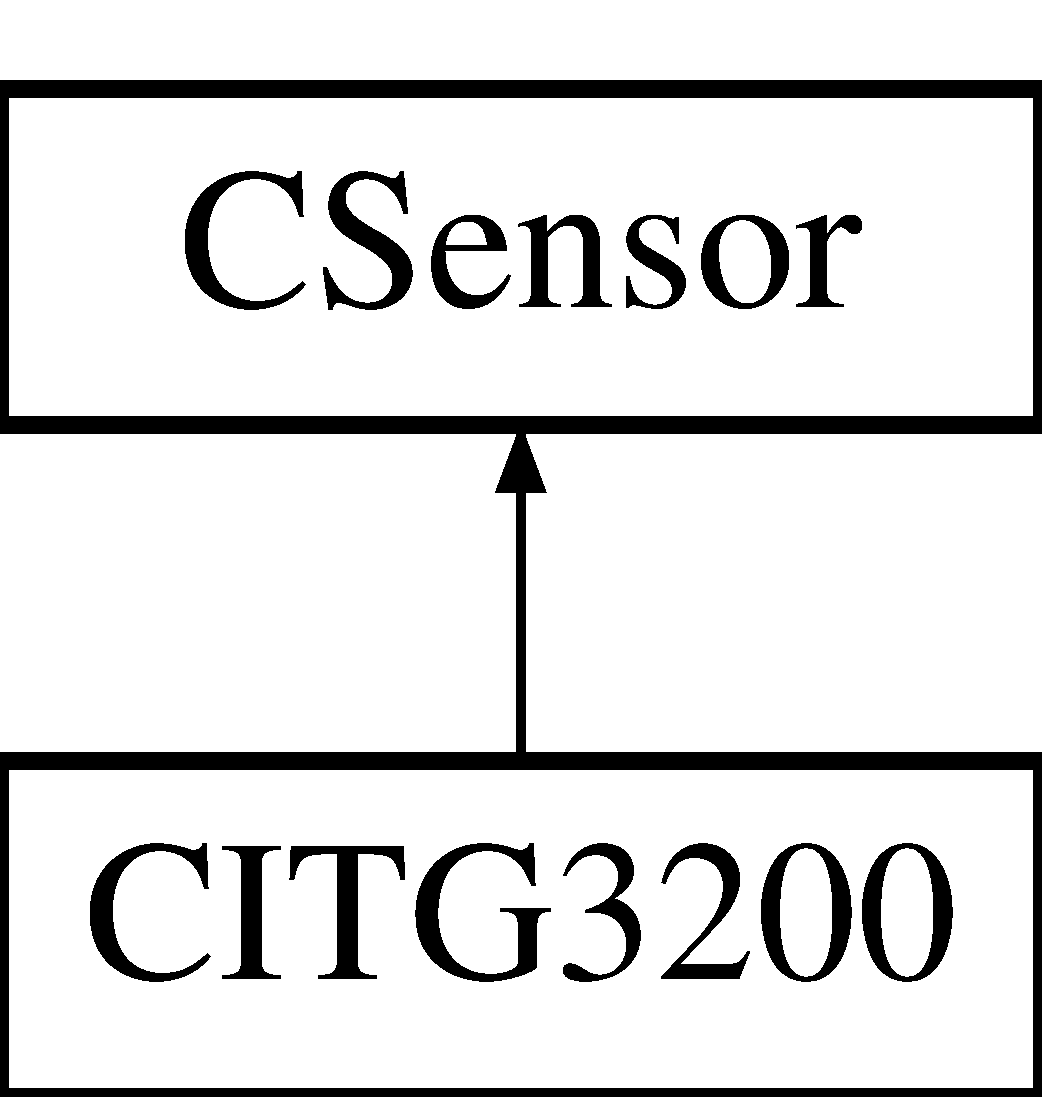
\includegraphics[height=2.000000cm]{class_c_i_t_g3200}
\end{center}
\end{figure}
\subsection*{Öffentliche \-Methoden}
\begin{DoxyCompactItemize}
\item 
\hypertarget{class_c_i_t_g3200_a3444eeb18a710346f95618264ca777be}{{\bfseries \-C\-I\-T\-G3200} (\hyperlink{class_c_i2_c}{\-C\-I2\-C} $\ast$p\-I2\-C, uint8\-\_\-t i\-Address)}\label{class_c_i_t_g3200_a3444eeb18a710346f95618264ca777be}

\item 
\hypertarget{class_c_i_t_g3200_a1f89d5f27aa435914ccb5bf821b1627c}{uint16\-\_\-t {\bfseries get\-Gyro\-X\-Raw} ()}\label{class_c_i_t_g3200_a1f89d5f27aa435914ccb5bf821b1627c}

\item 
\hypertarget{class_c_i_t_g3200_ac80a3dd95530de6ebdc11196f7d6b87f}{uint16\-\_\-t {\bfseries get\-Gyro\-Y\-Raw} ()}\label{class_c_i_t_g3200_ac80a3dd95530de6ebdc11196f7d6b87f}

\item 
\hypertarget{class_c_i_t_g3200_ae8ff101a3e68f6c607594666263e27f7}{uint16\-\_\-t {\bfseries get\-Gyro\-Z\-Raw} ()}\label{class_c_i_t_g3200_ae8ff101a3e68f6c607594666263e27f7}

\item 
\hypertarget{class_c_i_t_g3200_a1789a681319d8190770bce195bed22de}{float {\bfseries get\-Gyro\-X} ()}\label{class_c_i_t_g3200_a1789a681319d8190770bce195bed22de}

\item 
\hypertarget{class_c_i_t_g3200_acb51f15de2debbaf262ccd56aebff0dc}{float {\bfseries get\-Gyro\-Y} ()}\label{class_c_i_t_g3200_acb51f15de2debbaf262ccd56aebff0dc}

\item 
\hypertarget{class_c_i_t_g3200_a93b6f4ee7ba87f27d336f9e4e196e4b0}{float {\bfseries get\-Gyro\-Z} ()}\label{class_c_i_t_g3200_a93b6f4ee7ba87f27d336f9e4e196e4b0}

\item 
\hypertarget{class_c_i_t_g3200_a47d4044a6c4d6b4d197cc93da051c61b}{float {\bfseries get\-Gyro\-Alpha} ()}\label{class_c_i_t_g3200_a47d4044a6c4d6b4d197cc93da051c61b}

\item 
\hypertarget{class_c_i_t_g3200_abeba2a2808df982d93e4bdc98c8310eb}{float {\bfseries get\-Gyro\-Beta} ()}\label{class_c_i_t_g3200_abeba2a2808df982d93e4bdc98c8310eb}

\item 
\hypertarget{class_c_i_t_g3200_a918311e786932a6d7a3a51b2e3ab6377}{float {\bfseries get\-Gyro\-Gamma} ()}\label{class_c_i_t_g3200_a918311e786932a6d7a3a51b2e3ab6377}

\item 
\hypertarget{class_c_i_t_g3200_af4c5af49f17c7174d9690663258676a0}{\hyperlink{class_c_vector}{\-C\-Vector} {\bfseries get\-Gyro\-Vector} ()}\label{class_c_i_t_g3200_af4c5af49f17c7174d9690663258676a0}

\item 
\hypertarget{class_c_i_t_g3200_ab2bb903a4773f0d929c628e530add647}{uint16\-\_\-t {\bfseries get\-Gyro\-X\-Raw\-Per\-I2\-C} ()}\label{class_c_i_t_g3200_ab2bb903a4773f0d929c628e530add647}

\item 
\hypertarget{class_c_i_t_g3200_aef1d36d35a5550d333f5aa83b65da958}{uint16\-\_\-t {\bfseries get\-Gyro\-Y\-Raw\-Per\-I2\-C} ()}\label{class_c_i_t_g3200_aef1d36d35a5550d333f5aa83b65da958}

\item 
\hypertarget{class_c_i_t_g3200_aac22944a479b8cbdf2c45fccf1de5cdb}{uint16\-\_\-t {\bfseries get\-Gyro\-Z\-Raw\-Per\-I2\-C} ()}\label{class_c_i_t_g3200_aac22944a479b8cbdf2c45fccf1de5cdb}

\item 
\hypertarget{class_c_i_t_g3200_a6a796e117df241c1c40f478517ce8153}{float {\bfseries get\-Gyro\-X\-Per\-I2\-C} ()}\label{class_c_i_t_g3200_a6a796e117df241c1c40f478517ce8153}

\item 
\hypertarget{class_c_i_t_g3200_a9a42314e355fb3d2d3fb53b89903d08a}{float {\bfseries get\-Gyro\-Y\-Per\-I2\-C} ()}\label{class_c_i_t_g3200_a9a42314e355fb3d2d3fb53b89903d08a}

\item 
\hypertarget{class_c_i_t_g3200_aae0b7e8a0b79a573052e247dcc8b6d4c}{float {\bfseries get\-Gyro\-Z\-Per\-I2\-C} ()}\label{class_c_i_t_g3200_aae0b7e8a0b79a573052e247dcc8b6d4c}

\item 
\hypertarget{class_c_i_t_g3200_ae308a26abcf6b253e9ef44c7d38d3a32}{float {\bfseries get\-Gyro\-Alpha\-Per\-I2\-C} ()}\label{class_c_i_t_g3200_ae308a26abcf6b253e9ef44c7d38d3a32}

\item 
\hypertarget{class_c_i_t_g3200_a711f755203dbee78acac16b3b4e0cdbb}{float {\bfseries get\-Gyro\-Beta\-Per\-I2\-C} ()}\label{class_c_i_t_g3200_a711f755203dbee78acac16b3b4e0cdbb}

\item 
\hypertarget{class_c_i_t_g3200_a6a314af93c90ed6611727defb5258add}{float {\bfseries get\-Gyro\-Gamma\-Per\-I2\-C} ()}\label{class_c_i_t_g3200_a6a314af93c90ed6611727defb5258add}

\item 
\hypertarget{class_c_i_t_g3200_aca6c12f7d87787bfa17b9e48a8355ec7}{\hyperlink{class_c_vector}{\-C\-Vector} {\bfseries get\-Gyro\-Vector\-Per\-I2\-C} ()}\label{class_c_i_t_g3200_aca6c12f7d87787bfa17b9e48a8355ec7}

\item 
\hypertarget{class_c_i_t_g3200_a6233d13f5eb6ca6d38a81a7f8747a352}{void {\bfseries start} ()}\label{class_c_i_t_g3200_a6233d13f5eb6ca6d38a81a7f8747a352}

\item 
\hypertarget{class_c_i_t_g3200_ab101046e2977f9e5839e369dd024d4a9}{void {\bfseries stop} ()}\label{class_c_i_t_g3200_ab101046e2977f9e5839e369dd024d4a9}

\item 
\hypertarget{class_c_i_t_g3200_a69a8e093640f59d2c049d75806943382}{void {\bfseries kill} ()}\label{class_c_i_t_g3200_a69a8e093640f59d2c049d75806943382}

\item 
\hypertarget{class_c_i_t_g3200_ad9eca5440ccc683bc1dd882ab601986d}{void {\bfseries run} ()}\label{class_c_i_t_g3200_ad9eca5440ccc683bc1dd882ab601986d}

\item 
virtual bool \hyperlink{class_c_i_t_g3200_ae7b2da2eb5e8e7569e5b697db2124650}{get\-Value} (float \&i\-Value, uint8\-\_\-t i\-Channle)
\end{DoxyCompactItemize}


\subsection{\-Dokumentation der \-Elementfunktionen}
\hypertarget{class_c_i_t_g3200_ae7b2da2eb5e8e7569e5b697db2124650}{\index{\-C\-I\-T\-G3200@{\-C\-I\-T\-G3200}!get\-Value@{get\-Value}}
\index{get\-Value@{get\-Value}!CITG3200@{\-C\-I\-T\-G3200}}
\subsubsection[{get\-Value}]{\setlength{\rightskip}{0pt plus 5cm}virtual bool {\bf \-C\-I\-T\-G3200\-::get\-Value} (
\begin{DoxyParamCaption}
\item[{float \&}]{i\-Value, }
\item[{uint8\-\_\-t}]{i\-Channle}
\end{DoxyParamCaption}
)\hspace{0.3cm}{\ttfamily  \mbox{[}virtual\mbox{]}}}}\label{class_c_i_t_g3200_ae7b2da2eb5e8e7569e5b697db2124650}
\-Gibt den \-Wert i\-Value von dem \-Datenkanal i\-Channel zurück. 
\begin{DoxyParams}[1]{\-Parameter}
\mbox{\tt out}  & {\em i\-Value} & \-Wert der übergeben wird. \\
\hline
\mbox{\tt in}  & {\em i\-Channle} & \-Datenkanal von dem der \-Wert i\-Value übergeben werden soll. \\
\hline
\end{DoxyParams}
\begin{DoxyReturn}{\-Rückgabe}
\-Gibt zurück ob der \-Wert i\-Value von dem \-Datenkanal i\-Channle übergeben werden konnte, bzw. ob es den aufgerufenen \-Datenkanal gibt. 
\end{DoxyReturn}


\-Implementiert \hyperlink{class_c_sensor_a42b204fb320865a28b26478d079300d4}{\-C\-Sensor}.



\-Die \-Dokumentation für diese \-Klasse wurde erzeugt aufgrund der \-Datei\-:\begin{DoxyCompactItemize}
\item 
include/\-C\-I\-T\-G3200.\-h\end{DoxyCompactItemize}

\hypertarget{class_c_kalman_filter}{\section{\-C\-Kalman\-Filter \-Klassenreferenz}
\label{class_c_kalman_filter}\index{\-C\-Kalman\-Filter@{\-C\-Kalman\-Filter}}
}


\-Die \-Dokumentation für diese \-Klasse wurde erzeugt aufgrund der \-Datei\-:\begin{DoxyCompactItemize}
\item 
include/\-C\-Kalman\-Filter.\-h\end{DoxyCompactItemize}

\hypertarget{class_c_logger}{\section{\-C\-Logger \-Klassenreferenz}
\label{class_c_logger}\index{\-C\-Logger@{\-C\-Logger}}
}
\subsection*{Öffentliche \-Methoden}
\begin{DoxyCompactItemize}
\item 
\hypertarget{class_c_logger_ae6294be64612845abd2d5847cdd786e9}{{\bfseries \-C\-Logger} (const \hyperlink{class_c_logger}{\-C\-Logger} \&orig)}\label{class_c_logger_ae6294be64612845abd2d5847cdd786e9}

\end{DoxyCompactItemize}


\-Die \-Dokumentation für diese \-Klasse wurde erzeugt aufgrund der \-Datei\-:\begin{DoxyCompactItemize}
\item 
include/\-C\-Logger.\-h\end{DoxyCompactItemize}

\hypertarget{class_c_l_s_m303_d_l_h}{\section{\-C\-L\-S\-M303\-D\-L\-H \-Klassenreferenz}
\label{class_c_l_s_m303_d_l_h}\index{\-C\-L\-S\-M303\-D\-L\-H@{\-C\-L\-S\-M303\-D\-L\-H}}
}
\-Klassendiagramm für \-C\-L\-S\-M303\-D\-L\-H\-:\begin{figure}[H]
\begin{center}
\leavevmode
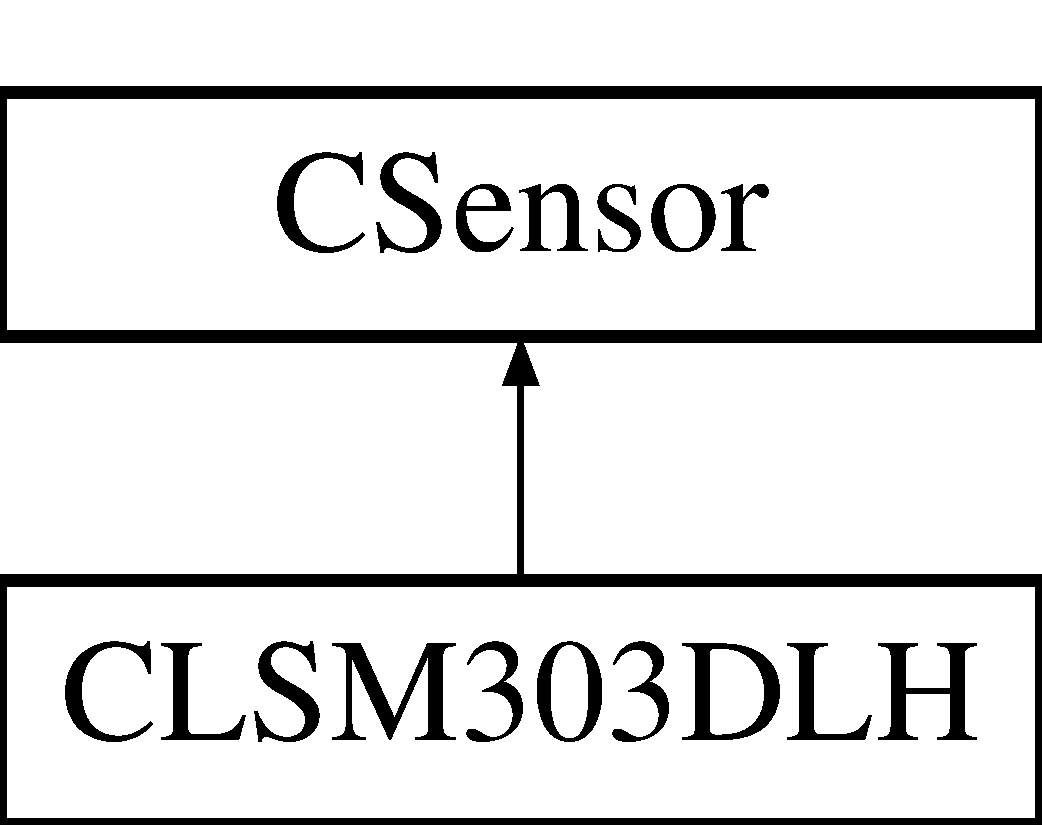
\includegraphics[height=2.000000cm]{class_c_l_s_m303_d_l_h}
\end{center}
\end{figure}
\subsection*{Öffentliche \-Methoden}
\begin{DoxyCompactItemize}
\item 
\hypertarget{class_c_l_s_m303_d_l_h_a02e1a3a5e5fe5d9c6656007c79bc94d0}{{\bfseries \-C\-L\-S\-M303\-D\-L\-H} (\hyperlink{class_c_i2_c}{\-C\-I2\-C} $\ast$p\-I2\-C, uint8\-\_\-t i\-Address)}\label{class_c_l_s_m303_d_l_h_a02e1a3a5e5fe5d9c6656007c79bc94d0}

\item 
\hypertarget{class_c_l_s_m303_d_l_h_a90eec511291bf7019dc48df6bca7aec8}{uint16\-\_\-t {\bfseries get\-Acc\-X\-Raw} ()}\label{class_c_l_s_m303_d_l_h_a90eec511291bf7019dc48df6bca7aec8}

\item 
\hypertarget{class_c_l_s_m303_d_l_h_ad4a82f3b958a42732a2acefc03728e67}{uint16\-\_\-t {\bfseries get\-Acc\-Y\-Raw} ()}\label{class_c_l_s_m303_d_l_h_ad4a82f3b958a42732a2acefc03728e67}

\item 
\hypertarget{class_c_l_s_m303_d_l_h_a776fae504ef79ba93b8c415b5ecde5ad}{uint16\-\_\-t {\bfseries get\-Acc\-Z\-Raw} ()}\label{class_c_l_s_m303_d_l_h_a776fae504ef79ba93b8c415b5ecde5ad}

\item 
\hypertarget{class_c_l_s_m303_d_l_h_a148c18e8e9f19107c0283d957b1091fb}{double {\bfseries get\-Acc\-X} ()}\label{class_c_l_s_m303_d_l_h_a148c18e8e9f19107c0283d957b1091fb}

\item 
\hypertarget{class_c_l_s_m303_d_l_h_ad8787615d5c0edb904155403e941c0c4}{double {\bfseries get\-Acc\-Y} ()}\label{class_c_l_s_m303_d_l_h_ad8787615d5c0edb904155403e941c0c4}

\item 
\hypertarget{class_c_l_s_m303_d_l_h_abf9d66bc467e3940a757f6ab300161b2}{double {\bfseries get\-Acc\-Z} ()}\label{class_c_l_s_m303_d_l_h_abf9d66bc467e3940a757f6ab300161b2}

\item 
\hypertarget{class_c_l_s_m303_d_l_h_a3848205668254941907cf808afac8c1e}{double {\bfseries get\-Acc\-Alpha} ()}\label{class_c_l_s_m303_d_l_h_a3848205668254941907cf808afac8c1e}

\item 
\hypertarget{class_c_l_s_m303_d_l_h_a9838438bcc4cc08c6543efac04b7f872}{double {\bfseries get\-Acc\-Beta} ()}\label{class_c_l_s_m303_d_l_h_a9838438bcc4cc08c6543efac04b7f872}

\item 
\hypertarget{class_c_l_s_m303_d_l_h_a3a3d0ed84f94a6c604337fa5a56a23ee}{double {\bfseries get\-Acc\-Gamma} ()}\label{class_c_l_s_m303_d_l_h_a3a3d0ed84f94a6c604337fa5a56a23ee}

\item 
\hypertarget{class_c_l_s_m303_d_l_h_a5a57c2b98bd1cc30b1d872e77a605883}{\hyperlink{class_c_vector}{\-C\-Vector} {\bfseries get\-Acc\-Vector} ()}\label{class_c_l_s_m303_d_l_h_a5a57c2b98bd1cc30b1d872e77a605883}

\item 
\hypertarget{class_c_l_s_m303_d_l_h_ab10666356085c61bb221adac6eec3f67}{uint16\-\_\-t {\bfseries get\-Acc\-X\-Raw\-Per\-I2\-C} ()}\label{class_c_l_s_m303_d_l_h_ab10666356085c61bb221adac6eec3f67}

\item 
\hypertarget{class_c_l_s_m303_d_l_h_a8b39f1059592bc437ff0a0076eee407b}{uint16\-\_\-t {\bfseries get\-Acc\-Y\-Raw\-Per\-I2\-C} ()}\label{class_c_l_s_m303_d_l_h_a8b39f1059592bc437ff0a0076eee407b}

\item 
\hypertarget{class_c_l_s_m303_d_l_h_a8601bc0c40673413fd508609bf4c97b9}{uint16\-\_\-t {\bfseries get\-Acc\-Z\-Raw\-Per\-I2\-C} ()}\label{class_c_l_s_m303_d_l_h_a8601bc0c40673413fd508609bf4c97b9}

\item 
\hypertarget{class_c_l_s_m303_d_l_h_a43afbef561eb5c77bd68ca23c74d142a}{double {\bfseries get\-Acc\-X\-Per\-I2\-C} ()}\label{class_c_l_s_m303_d_l_h_a43afbef561eb5c77bd68ca23c74d142a}

\item 
\hypertarget{class_c_l_s_m303_d_l_h_a010b3bbd9dcb4a9162201b4086ca4694}{double {\bfseries get\-Acc\-Y\-Per\-I2\-C} ()}\label{class_c_l_s_m303_d_l_h_a010b3bbd9dcb4a9162201b4086ca4694}

\item 
\hypertarget{class_c_l_s_m303_d_l_h_a7ace98c523c1b94763c1ba5eb62d0b2a}{double {\bfseries get\-Acc\-Z\-Per\-I2\-C} ()}\label{class_c_l_s_m303_d_l_h_a7ace98c523c1b94763c1ba5eb62d0b2a}

\item 
\hypertarget{class_c_l_s_m303_d_l_h_a4e7bc204a848a50de8cebb3c9441deeb}{double {\bfseries get\-Acc\-Alpha\-Per\-I2\-C} ()}\label{class_c_l_s_m303_d_l_h_a4e7bc204a848a50de8cebb3c9441deeb}

\item 
\hypertarget{class_c_l_s_m303_d_l_h_a5625048bf3bc05521f2e2a8758c46c71}{double {\bfseries get\-Acc\-Beta\-Per\-I2\-C} ()}\label{class_c_l_s_m303_d_l_h_a5625048bf3bc05521f2e2a8758c46c71}

\item 
\hypertarget{class_c_l_s_m303_d_l_h_a270276cd54b79ad07f337e6a726b5215}{double {\bfseries get\-Acc\-Gamma\-Per\-I2\-C} ()}\label{class_c_l_s_m303_d_l_h_a270276cd54b79ad07f337e6a726b5215}

\item 
\hypertarget{class_c_l_s_m303_d_l_h_abd6a8143e89616462de605234ce5543d}{\hyperlink{class_c_vector}{\-C\-Vector} {\bfseries get\-Acc\-Vector\-Per\-I2\-C} ()}\label{class_c_l_s_m303_d_l_h_abd6a8143e89616462de605234ce5543d}

\item 
\hypertarget{class_c_l_s_m303_d_l_h_af3e1ff4f8bc6e7943e138bca7024034b}{uint16\-\_\-t {\bfseries get\-Mag\-X\-Raw} ()}\label{class_c_l_s_m303_d_l_h_af3e1ff4f8bc6e7943e138bca7024034b}

\item 
\hypertarget{class_c_l_s_m303_d_l_h_ab512f2eb8d5768f3c319fad11e855fe3}{uint16\-\_\-t {\bfseries get\-Mag\-Y\-Raw} ()}\label{class_c_l_s_m303_d_l_h_ab512f2eb8d5768f3c319fad11e855fe3}

\item 
\hypertarget{class_c_l_s_m303_d_l_h_ab111107af5f8bdf720039ecbb3d7c3a6}{uint16\-\_\-t {\bfseries get\-Mag\-Z\-Raw} ()}\label{class_c_l_s_m303_d_l_h_ab111107af5f8bdf720039ecbb3d7c3a6}

\item 
\hypertarget{class_c_l_s_m303_d_l_h_a2bfb4713dccaa2c3da90961d62b62384}{double {\bfseries get\-Mag\-X} ()}\label{class_c_l_s_m303_d_l_h_a2bfb4713dccaa2c3da90961d62b62384}

\item 
\hypertarget{class_c_l_s_m303_d_l_h_ac42bacf557ecb97ea1cb4499d998a67f}{double {\bfseries get\-Mag\-Y} ()}\label{class_c_l_s_m303_d_l_h_ac42bacf557ecb97ea1cb4499d998a67f}

\item 
\hypertarget{class_c_l_s_m303_d_l_h_aa130822b3b5d971e6701c6866ad2e8e6}{double {\bfseries get\-Mag\-Z} ()}\label{class_c_l_s_m303_d_l_h_aa130822b3b5d971e6701c6866ad2e8e6}

\item 
\hypertarget{class_c_l_s_m303_d_l_h_af8aa6f1e3a2da5e1895691316b2650e2}{double {\bfseries get\-Mag\-Alpha} ()}\label{class_c_l_s_m303_d_l_h_af8aa6f1e3a2da5e1895691316b2650e2}

\item 
\hypertarget{class_c_l_s_m303_d_l_h_a1706e7e8bef14ed8e279e992793a25ed}{double {\bfseries get\-Mag\-Beta} ()}\label{class_c_l_s_m303_d_l_h_a1706e7e8bef14ed8e279e992793a25ed}

\item 
\hypertarget{class_c_l_s_m303_d_l_h_a3ea17cdda5d2028aec077f33884b4ea9}{double {\bfseries get\-Mag\-Gamma} ()}\label{class_c_l_s_m303_d_l_h_a3ea17cdda5d2028aec077f33884b4ea9}

\item 
\hypertarget{class_c_l_s_m303_d_l_h_a19c402f7d403ae2014ee3077dbd16236}{\hyperlink{class_c_vector}{\-C\-Vector} {\bfseries get\-Mag\-Vector} ()}\label{class_c_l_s_m303_d_l_h_a19c402f7d403ae2014ee3077dbd16236}

\item 
\hypertarget{class_c_l_s_m303_d_l_h_aec2605d44808d1695b9fc433a9c396a8}{uint16\-\_\-t {\bfseries get\-Mag\-X\-Raw\-Per\-I2\-C} ()}\label{class_c_l_s_m303_d_l_h_aec2605d44808d1695b9fc433a9c396a8}

\item 
\hypertarget{class_c_l_s_m303_d_l_h_aa606744506c0062c73ab2bb4257bca97}{uint16\-\_\-t {\bfseries get\-Mag\-Y\-Raw\-Per\-I2\-C} ()}\label{class_c_l_s_m303_d_l_h_aa606744506c0062c73ab2bb4257bca97}

\item 
\hypertarget{class_c_l_s_m303_d_l_h_ad14d66c995b152040823b68fbae7a674}{uint16\-\_\-t {\bfseries get\-Mag\-Z\-Raw\-Per\-I2\-C} ()}\label{class_c_l_s_m303_d_l_h_ad14d66c995b152040823b68fbae7a674}

\item 
\hypertarget{class_c_l_s_m303_d_l_h_a05c0feec299de3eab196bc32fe74773f}{double {\bfseries get\-Mag\-X\-Per\-I2\-C} ()}\label{class_c_l_s_m303_d_l_h_a05c0feec299de3eab196bc32fe74773f}

\item 
\hypertarget{class_c_l_s_m303_d_l_h_aa425ba55feb791235568e746b4208ac1}{double {\bfseries get\-Mag\-Y\-Per\-I2\-C} ()}\label{class_c_l_s_m303_d_l_h_aa425ba55feb791235568e746b4208ac1}

\item 
\hypertarget{class_c_l_s_m303_d_l_h_ad3bf467e8579b7ab545b7aad6ba2a025}{double {\bfseries get\-Mag\-Z\-Per\-I2\-C} ()}\label{class_c_l_s_m303_d_l_h_ad3bf467e8579b7ab545b7aad6ba2a025}

\item 
\hypertarget{class_c_l_s_m303_d_l_h_a1ea462a9ed3b9014f96c63f67fd2cd08}{double {\bfseries get\-Mag\-Alpha\-Per\-I2\-C} ()}\label{class_c_l_s_m303_d_l_h_a1ea462a9ed3b9014f96c63f67fd2cd08}

\item 
\hypertarget{class_c_l_s_m303_d_l_h_aa39de2e0f08f9986dbd1262320c9d1ee}{double {\bfseries get\-Mag\-Beta\-Per\-I2\-C} ()}\label{class_c_l_s_m303_d_l_h_aa39de2e0f08f9986dbd1262320c9d1ee}

\item 
\hypertarget{class_c_l_s_m303_d_l_h_a2155291a89ad187bb2e1c1ca347d925f}{double {\bfseries get\-Mag\-Gamma\-Per\-I2\-C} ()}\label{class_c_l_s_m303_d_l_h_a2155291a89ad187bb2e1c1ca347d925f}

\item 
\hypertarget{class_c_l_s_m303_d_l_h_a3ed857be8913e6f5beda82a3cfefe1d2}{\hyperlink{class_c_vector}{\-C\-Vector} {\bfseries get\-Mag\-Vector\-Per\-I2\-C} ()}\label{class_c_l_s_m303_d_l_h_a3ed857be8913e6f5beda82a3cfefe1d2}

\item 
\hypertarget{class_c_l_s_m303_d_l_h_a847e9a0faff128c259f91ecdc4c47745}{void {\bfseries start} ()}\label{class_c_l_s_m303_d_l_h_a847e9a0faff128c259f91ecdc4c47745}

\item 
\hypertarget{class_c_l_s_m303_d_l_h_af5947cac08ab6246a93c73a8d45334de}{void {\bfseries stop} ()}\label{class_c_l_s_m303_d_l_h_af5947cac08ab6246a93c73a8d45334de}

\item 
\hypertarget{class_c_l_s_m303_d_l_h_ac9ea19f2def71b8605cf0fa9a554e7fe}{void {\bfseries kill} ()}\label{class_c_l_s_m303_d_l_h_ac9ea19f2def71b8605cf0fa9a554e7fe}

\item 
\hypertarget{class_c_l_s_m303_d_l_h_acab2194faf7332d8209e30a0fb397288}{void {\bfseries run} ()}\label{class_c_l_s_m303_d_l_h_acab2194faf7332d8209e30a0fb397288}

\item 
\hypertarget{class_c_l_s_m303_d_l_h_a58a58643906cee882a3e77ec9e733032}{virtual int8\-\_\-t {\bfseries get\-Value} (int16\-\_\-t \&i\-Value, uint8\-\_\-t i\-Channle)}\label{class_c_l_s_m303_d_l_h_a58a58643906cee882a3e77ec9e733032}

\end{DoxyCompactItemize}


\-Die \-Dokumentation für diese \-Klasse wurde erzeugt aufgrund der \-Datei\-:\begin{DoxyCompactItemize}
\item 
include/\-C\-L\-S\-M303\-D\-L\-H.\-h\end{DoxyCompactItemize}

\hypertarget{class_c_motor}{\section{\-C\-Motor \-Klassenreferenz}
\label{class_c_motor}\index{\-C\-Motor@{\-C\-Motor}}
}
\-Klassendiagramm für \-C\-Motor\-:\begin{figure}[H]
\begin{center}
\leavevmode
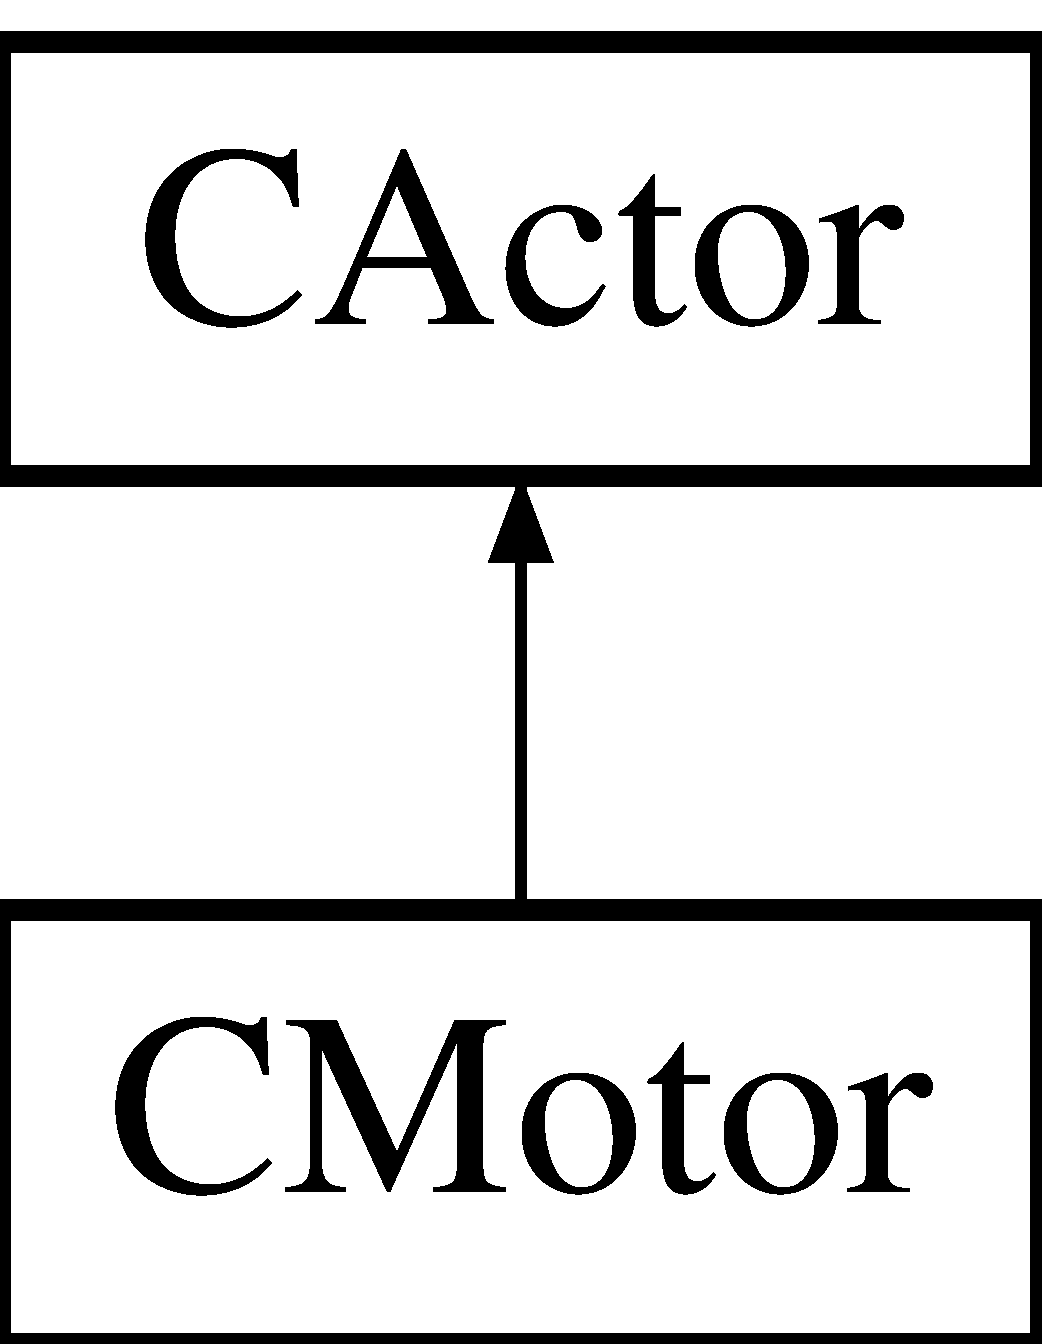
\includegraphics[height=2.000000cm]{class_c_motor}
\end{center}
\end{figure}
\subsection*{Öffentliche \-Methoden}
\begin{DoxyCompactItemize}
\item 
\hypertarget{class_c_motor_a5f57ccb412c2fed1ab8737635bc792d7}{{\bfseries \-C\-Motor} (\hyperlink{class_c_p_w_m_driver}{\-C\-P\-W\-M\-Driver} $\ast$p\-P\-W\-M\-Driver, uint8\-\_\-t i\-Channle)}\label{class_c_motor_a5f57ccb412c2fed1ab8737635bc792d7}

\item 
\hypertarget{class_c_motor_ae25560c278459aae37e4299e0b4dfca0}{void {\bfseries set\-Speed} (int16\-\_\-t i\-Speed)}\label{class_c_motor_ae25560c278459aae37e4299e0b4dfca0}

\item 
\hypertarget{class_c_motor_ae34038ec0b69bc46462e706ca9fa9454}{int16\-\_\-t {\bfseries get\-Speed} ()}\label{class_c_motor_ae34038ec0b69bc46462e706ca9fa9454}

\item 
\hypertarget{class_c_motor_acaf02cf61cb003e1d675c696a1411df1}{void {\bfseries stop} ()}\label{class_c_motor_acaf02cf61cb003e1d675c696a1411df1}

\item 
virtual bool \hyperlink{class_c_motor_a83fa60cbf910c7386fb45db8ea875de1}{set\-Value} (float i\-Value, uint8\-\_\-t i\-Channle)
\end{DoxyCompactItemize}


\subsection{\-Dokumentation der \-Elementfunktionen}
\hypertarget{class_c_motor_a83fa60cbf910c7386fb45db8ea875de1}{\index{\-C\-Motor@{\-C\-Motor}!set\-Value@{set\-Value}}
\index{set\-Value@{set\-Value}!CMotor@{\-C\-Motor}}
\subsubsection[{set\-Value}]{\setlength{\rightskip}{0pt plus 5cm}virtual bool {\bf \-C\-Motor\-::set\-Value} (
\begin{DoxyParamCaption}
\item[{float}]{i\-Value, }
\item[{uint8\-\_\-t}]{i\-Channle}
\end{DoxyParamCaption}
)\hspace{0.3cm}{\ttfamily  \mbox{[}virtual\mbox{]}}}}\label{class_c_motor_a83fa60cbf910c7386fb45db8ea875de1}
\-Gibt den \-Wert i\-Value an den \-Datenkanal i\-Channel weiter. 
\begin{DoxyParams}[1]{\-Parameter}
\mbox{\tt in}  & {\em i\-Value} & \-Wert der übergeben werden soll. \\
\hline
\mbox{\tt in}  & {\em i\-Channle} & \-Datenkanal an dem der \-Wert i\-Value übergeben werden soll. \\
\hline
\end{DoxyParams}
\begin{DoxyReturn}{\-Rückgabe}
\-Gibt zurück ob der \-Wert i\-Value in den \-Datenkanal i\-Channle übergeben werden konnte, bzw. ob es den aufgerufenen \-Datenkanal gibt. 
\end{DoxyReturn}


\-Implementiert \hyperlink{class_c_actor_a8a04a31e44aaa861d97bdbeb7ae1a570}{\-C\-Actor}.



\-Die \-Dokumentation für diese \-Klasse wurde erzeugt aufgrund der \-Datei\-:\begin{DoxyCompactItemize}
\item 
include/\-C\-Motor.\-h\end{DoxyCompactItemize}

\hypertarget{class_c_p_i_d_regler}{\section{\-C\-P\-I\-D\-Regler \-Klassenreferenz}
\label{class_c_p_i_d_regler}\index{\-C\-P\-I\-D\-Regler@{\-C\-P\-I\-D\-Regler}}
}
\subsection*{Öffentliche \-Methoden}
\begin{DoxyCompactItemize}
\item 
\hypertarget{class_c_p_i_d_regler_aba10334ff96913dd5b4897bf66f180b3}{{\bfseries \-C\-P\-I\-D\-Regler} (\hyperlink{class_c_sensor}{\-C\-Sensor} $\ast$p\-Sensor, uint8\-\_\-t i\-Sensor\-Channle, \hyperlink{class_c_actor}{\-C\-Actor} $\ast$p\-Actor, uint8\-\_\-t i\-Actor\-Channle)}\label{class_c_p_i_d_regler_aba10334ff96913dd5b4897bf66f180b3}

\item 
\hypertarget{class_c_p_i_d_regler_a907fe2535c7e05c8e5696e4e2d2f2c12}{void {\bfseries set\-Soll} (float soll)}\label{class_c_p_i_d_regler_a907fe2535c7e05c8e5696e4e2d2f2c12}

\item 
\hypertarget{class_c_p_i_d_regler_a7dad8bea3f3437fa6eb2a3d3d6b7e4ca}{void {\bfseries set\-Kp} (float \-Kp)}\label{class_c_p_i_d_regler_a7dad8bea3f3437fa6eb2a3d3d6b7e4ca}

\item 
\hypertarget{class_c_p_i_d_regler_a0fd9b03d63acba128df6a42ae3912102}{void {\bfseries set\-Ki} (float \-Ki)}\label{class_c_p_i_d_regler_a0fd9b03d63acba128df6a42ae3912102}

\item 
\hypertarget{class_c_p_i_d_regler_a75f7733582c014ec2d0a39e974635060}{void {\bfseries set\-Kd} (float \-Kd)}\label{class_c_p_i_d_regler_a75f7733582c014ec2d0a39e974635060}

\item 
\hypertarget{class_c_p_i_d_regler_a70cfefe00f0d6624fb3a8ea826b29ea9}{void {\bfseries set\-Time} (uint16\-\_\-t i\-Time)}\label{class_c_p_i_d_regler_a70cfefe00f0d6624fb3a8ea826b29ea9}

\item 
\hypertarget{class_c_p_i_d_regler_ac3bfef2e23e79b195d4e0726ea96524c}{float {\bfseries get\-Kp} ()}\label{class_c_p_i_d_regler_ac3bfef2e23e79b195d4e0726ea96524c}

\item 
\hypertarget{class_c_p_i_d_regler_aa9200343d94310765d4d6e6ba8b6bb30}{float {\bfseries get\-Ki} ()}\label{class_c_p_i_d_regler_aa9200343d94310765d4d6e6ba8b6bb30}

\item 
\hypertarget{class_c_p_i_d_regler_ac7407cdca458abb7fb830edd87ae8748}{float {\bfseries get\-Kd} ()}\label{class_c_p_i_d_regler_ac7407cdca458abb7fb830edd87ae8748}

\item 
\hypertarget{class_c_p_i_d_regler_a7785f43ec48ca84323ada78d27af45f1}{uint16\-\_\-t {\bfseries get\-Time} ()}\label{class_c_p_i_d_regler_a7785f43ec48ca84323ada78d27af45f1}

\item 
\hypertarget{class_c_p_i_d_regler_a78cbfbd338c7608b070397b9658911cb}{void {\bfseries start} ()}\label{class_c_p_i_d_regler_a78cbfbd338c7608b070397b9658911cb}

\item 
\hypertarget{class_c_p_i_d_regler_a04dd1b9a412f5bfaa6741d3354b1fe69}{void {\bfseries stop} ()}\label{class_c_p_i_d_regler_a04dd1b9a412f5bfaa6741d3354b1fe69}

\item 
\hypertarget{class_c_p_i_d_regler_a50419ad1c3923f7e7d8b67dc17f5cf24}{void {\bfseries kill} ()}\label{class_c_p_i_d_regler_a50419ad1c3923f7e7d8b67dc17f5cf24}

\item 
\hypertarget{class_c_p_i_d_regler_a92cbd69baca2de5c4cb57b43e47e14cf}{void {\bfseries run} ()}\label{class_c_p_i_d_regler_a92cbd69baca2de5c4cb57b43e47e14cf}

\end{DoxyCompactItemize}


\-Die \-Dokumentation für diese \-Klasse wurde erzeugt aufgrund der \-Datei\-:\begin{DoxyCompactItemize}
\item 
include/\-C\-P\-I\-D\-Regler.\-h\end{DoxyCompactItemize}

\hypertarget{class_c_p_w_m}{\section{\-C\-P\-W\-M \-Klassenreferenz}
\label{class_c_p_w_m}\index{\-C\-P\-W\-M@{\-C\-P\-W\-M}}
}
\subsection*{Öffentliche \-Methoden}
\begin{DoxyCompactItemize}
\item 
\hypertarget{class_c_p_w_m_aacaf1dfa5e9674249dfe0a2ed5753e4d}{{\bfseries \-C\-P\-W\-M} (const \hyperlink{class_c_p_w_m}{\-C\-P\-W\-M} \&orig)}\label{class_c_p_w_m_aacaf1dfa5e9674249dfe0a2ed5753e4d}

\end{DoxyCompactItemize}


\-Die \-Dokumentation für diese \-Klasse wurde erzeugt aufgrund der \-Datei\-:\begin{DoxyCompactItemize}
\item 
include/\-C\-P\-W\-M.\-h\end{DoxyCompactItemize}

\hypertarget{class_c_p_w_m_driver}{\section{\-C\-P\-W\-M\-Driver \-Klassenreferenz}
\label{class_c_p_w_m_driver}\index{\-C\-P\-W\-M\-Driver@{\-C\-P\-W\-M\-Driver}}
}
\-Klassendiagramm für \-C\-P\-W\-M\-Driver\-:\begin{figure}[H]
\begin{center}
\leavevmode
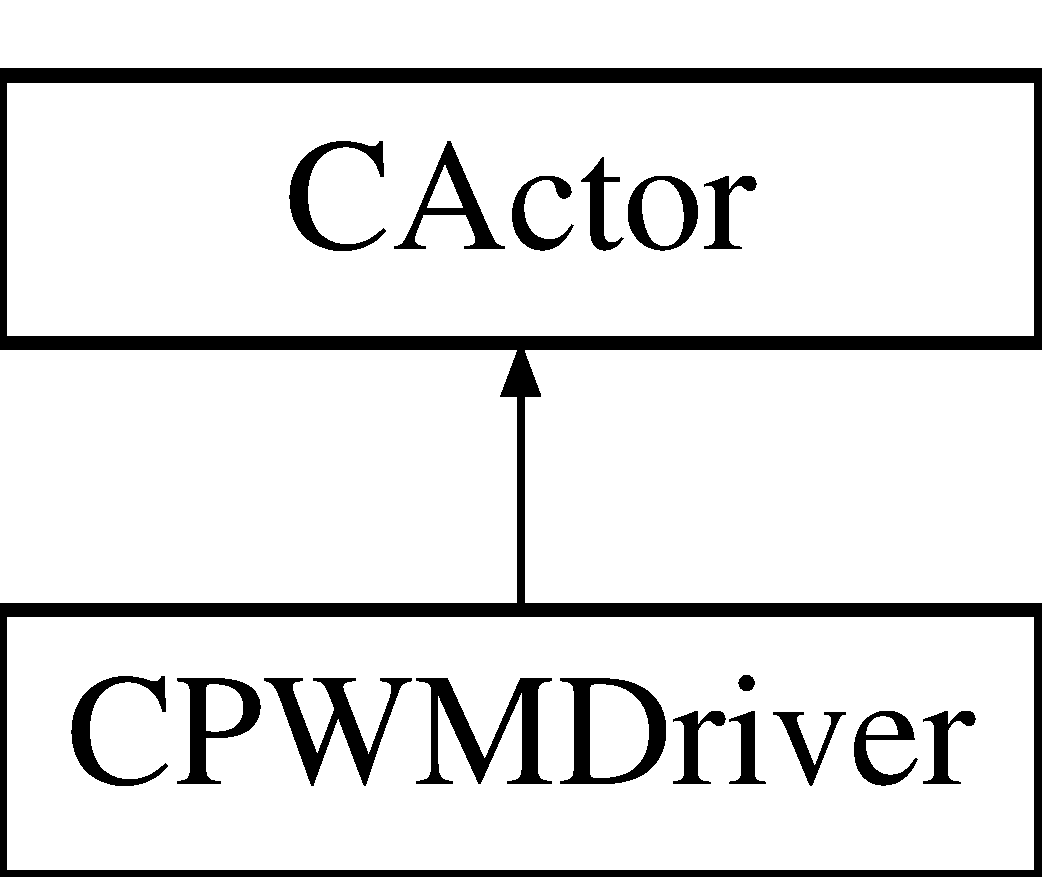
\includegraphics[height=2.000000cm]{class_c_p_w_m_driver}
\end{center}
\end{figure}
\subsection*{Öffentliche \-Methoden}
\begin{DoxyCompactItemize}
\item 
\hypertarget{class_c_p_w_m_driver_a0ce7f67c234b48d234c3c7bcc4aaef62}{{\bfseries \-C\-P\-W\-M\-Driver} (\hyperlink{class_c_i2_c}{\-C\-I2\-C} $\ast$p\-I2\-C, uint8\-\_\-t i\-Address)}\label{class_c_p_w_m_driver_a0ce7f67c234b48d234c3c7bcc4aaef62}

\item 
\hypertarget{class_c_p_w_m_driver_a8d4599eac8535a08204a2a7a53c882fe}{void {\bfseries set\-P\-W\-M} (uint8\-\_\-t i\-Channle, uint16\-\_\-t i\-Duty\-Cycle)}\label{class_c_p_w_m_driver_a8d4599eac8535a08204a2a7a53c882fe}

\item 
\hypertarget{class_c_p_w_m_driver_ae8945a237fd6e4f5dfc68f867a7c8c43}{void {\bfseries set\-Period} (uint16\-\_\-t i\-Period\-Time)}\label{class_c_p_w_m_driver_ae8945a237fd6e4f5dfc68f867a7c8c43}

\item 
\hypertarget{class_c_p_w_m_driver_ad373149ae4a7047f6e38a372ab6cb446}{uint16\-\_\-t {\bfseries get\-P\-W\-M} (uint8\-\_\-t i\-C\-Hannle)}\label{class_c_p_w_m_driver_ad373149ae4a7047f6e38a372ab6cb446}

\item 
\hypertarget{class_c_p_w_m_driver_a021de939d6d981c6b961403943e58dd9}{uint16\-\_\-t {\bfseries get\-Period} ()}\label{class_c_p_w_m_driver_a021de939d6d981c6b961403943e58dd9}

\item 
virtual bool \hyperlink{class_c_p_w_m_driver_a91a128c891a11d64ba7a8d1486e77fab}{set\-Value} (float i\-Value, uint8\-\_\-t i\-Channle)
\end{DoxyCompactItemize}


\subsection{\-Dokumentation der \-Elementfunktionen}
\hypertarget{class_c_p_w_m_driver_a91a128c891a11d64ba7a8d1486e77fab}{\index{\-C\-P\-W\-M\-Driver@{\-C\-P\-W\-M\-Driver}!set\-Value@{set\-Value}}
\index{set\-Value@{set\-Value}!CPWMDriver@{\-C\-P\-W\-M\-Driver}}
\subsubsection[{set\-Value}]{\setlength{\rightskip}{0pt plus 5cm}virtual bool {\bf \-C\-P\-W\-M\-Driver\-::set\-Value} (
\begin{DoxyParamCaption}
\item[{float}]{i\-Value, }
\item[{uint8\-\_\-t}]{i\-Channle}
\end{DoxyParamCaption}
)\hspace{0.3cm}{\ttfamily  \mbox{[}virtual\mbox{]}}}}\label{class_c_p_w_m_driver_a91a128c891a11d64ba7a8d1486e77fab}
\-Gibt den \-Wert i\-Value an den \-Datenkanal i\-Channel weiter. 
\begin{DoxyParams}[1]{\-Parameter}
\mbox{\tt in}  & {\em i\-Value} & \-Wert der übergeben werden soll. \\
\hline
\mbox{\tt in}  & {\em i\-Channle} & \-Datenkanal an dem der \-Wert i\-Value übergeben werden soll. \\
\hline
\end{DoxyParams}
\begin{DoxyReturn}{\-Rückgabe}
\-Gibt zurück ob der \-Wert i\-Value in den \-Datenkanal i\-Channle übergeben werden konnte, bzw. ob es den aufgerufenen \-Datenkanal gibt. 
\end{DoxyReturn}


\-Implementiert \hyperlink{class_c_actor_a8a04a31e44aaa861d97bdbeb7ae1a570}{\-C\-Actor}.



\-Die \-Dokumentation für diese \-Klasse wurde erzeugt aufgrund der \-Datei\-:\begin{DoxyCompactItemize}
\item 
include/\-C\-P\-W\-M\-Driver.\-h\end{DoxyCompactItemize}

\hypertarget{class_c_r_p_meter}{\section{\-C\-R\-P\-Meter \-Klassenreferenz}
\label{class_c_r_p_meter}\index{\-C\-R\-P\-Meter@{\-C\-R\-P\-Meter}}
}
\-Klassendiagramm für \-C\-R\-P\-Meter\-:\begin{figure}[H]
\begin{center}
\leavevmode
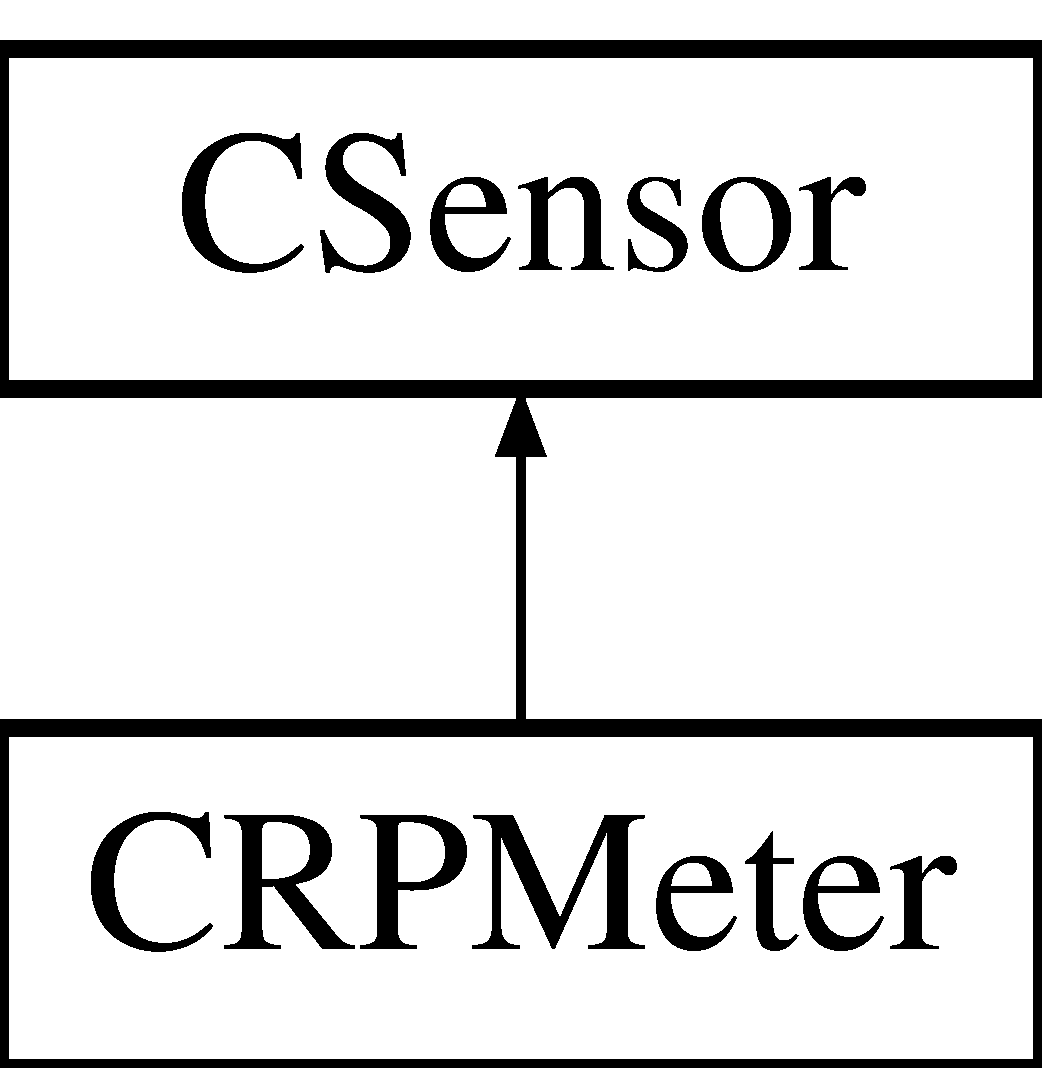
\includegraphics[height=2.000000cm]{class_c_r_p_meter}
\end{center}
\end{figure}
\subsection*{Öffentliche \-Methoden}
\begin{DoxyCompactItemize}
\item 
\hypertarget{class_c_r_p_meter_ab0ce8f26cfa08edfe5f8b0810591eaca}{{\bfseries \-C\-R\-P\-Meter} (\hyperlink{class_c_i2_c}{\-C\-I2\-C} $\ast$p\-I2\-C, uint8\-\_\-t i\-Address)}\label{class_c_r_p_meter_ab0ce8f26cfa08edfe5f8b0810591eaca}

\item 
\hypertarget{class_c_r_p_meter_ae777168160c21ca61fcc2070bd691ef6}{void {\bfseries start} ()}\label{class_c_r_p_meter_ae777168160c21ca61fcc2070bd691ef6}

\item 
\hypertarget{class_c_r_p_meter_a2af8f07faa15457ab5440eed411065e5}{void {\bfseries stop} ()}\label{class_c_r_p_meter_a2af8f07faa15457ab5440eed411065e5}

\item 
\hypertarget{class_c_r_p_meter_a866096ac582ba8d3a743644dcfb25839}{void {\bfseries kill} ()}\label{class_c_r_p_meter_a866096ac582ba8d3a743644dcfb25839}

\item 
\hypertarget{class_c_r_p_meter_a54f8a5a721ce32a3557383429af33308}{void {\bfseries run} ()}\label{class_c_r_p_meter_a54f8a5a721ce32a3557383429af33308}

\item 
virtual bool \hyperlink{class_c_r_p_meter_af0c4786702d4abda2f61b0b0f9c968fa}{get\-Value} (float \&i\-Value, uint8\-\_\-t i\-Channle)
\end{DoxyCompactItemize}


\subsection{\-Dokumentation der \-Elementfunktionen}
\hypertarget{class_c_r_p_meter_af0c4786702d4abda2f61b0b0f9c968fa}{\index{\-C\-R\-P\-Meter@{\-C\-R\-P\-Meter}!get\-Value@{get\-Value}}
\index{get\-Value@{get\-Value}!CRPMeter@{\-C\-R\-P\-Meter}}
\subsubsection[{get\-Value}]{\setlength{\rightskip}{0pt plus 5cm}virtual bool {\bf \-C\-R\-P\-Meter\-::get\-Value} (
\begin{DoxyParamCaption}
\item[{float \&}]{i\-Value, }
\item[{uint8\-\_\-t}]{i\-Channle}
\end{DoxyParamCaption}
)\hspace{0.3cm}{\ttfamily  \mbox{[}virtual\mbox{]}}}}\label{class_c_r_p_meter_af0c4786702d4abda2f61b0b0f9c968fa}
\-Gibt den \-Wert i\-Value von dem \-Datenkanal i\-Channel zurück. 
\begin{DoxyParams}[1]{\-Parameter}
\mbox{\tt out}  & {\em i\-Value} & \-Wert der zurückgegeben wird. \\
\hline
\mbox{\tt in}  & {\em i\-Channle} & \-Datenkanal von dem der \-Wert i\-Value übergeben werden soll. \\
\hline
\end{DoxyParams}
\begin{DoxyReturn}{\-Rückgabe}
\-Gibt zurück ob der \-Wert i\-Value von dem \-Datenkanal i\-Channle übergeben werden konnte, bzw. ob es den aufgerufenen \-Datenkanal gibt. 
\end{DoxyReturn}


\-Implementiert \hyperlink{class_c_sensor_a42b204fb320865a28b26478d079300d4}{\-C\-Sensor}.



\-Die \-Dokumentation für diese \-Klasse wurde erzeugt aufgrund der \-Datei\-:\begin{DoxyCompactItemize}
\item 
include/\-C\-R\-P\-Meter.\-h\end{DoxyCompactItemize}

\hypertarget{class_c_sensor}{\section{\-C\-Sensor \-Klassenreferenz}
\label{class_c_sensor}\index{\-C\-Sensor@{\-C\-Sensor}}
}
\-Klassendiagramm für \-C\-Sensor\-:\begin{figure}[H]
\begin{center}
\leavevmode
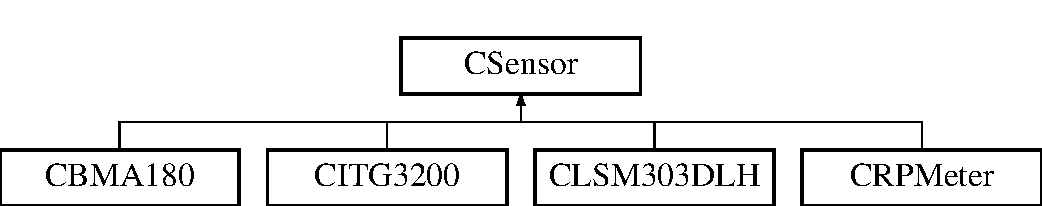
\includegraphics[height=2.000000cm]{class_c_sensor}
\end{center}
\end{figure}
\subsection*{Öffentliche \-Methoden}
\begin{DoxyCompactItemize}
\item 
\hyperlink{class_c_sensor_ac1bb4774cc283d52efc154b0a3ce015b}{\-C\-Sensor} ()
\item 
virtual \hyperlink{class_c_sensor_ae055a59cd5010662761925d24d174004}{$\sim$\-C\-Sensor} ()
\item 
virtual bool \hyperlink{class_c_sensor_a42b204fb320865a28b26478d079300d4}{get\-Value} (float \&i\-Value, uint8\-\_\-t i\-Channle)=0
\end{DoxyCompactItemize}


\subsection{\-Beschreibung der \-Konstruktoren und \-Destruktoren}
\hypertarget{class_c_sensor_ac1bb4774cc283d52efc154b0a3ce015b}{\index{\-C\-Sensor@{\-C\-Sensor}!\-C\-Sensor@{\-C\-Sensor}}
\index{\-C\-Sensor@{\-C\-Sensor}!CSensor@{\-C\-Sensor}}
\subsubsection[{\-C\-Sensor}]{\setlength{\rightskip}{0pt plus 5cm}{\bf \-C\-Sensor\-::\-C\-Sensor} (
\begin{DoxyParamCaption}
{}
\end{DoxyParamCaption}
)}}\label{class_c_sensor_ac1bb4774cc283d52efc154b0a3ce015b}
\-Erzeugt ein \-Objekt der \-Klasse \hyperlink{class_c_sensor}{\-C\-Sensor}. \hypertarget{class_c_sensor_ae055a59cd5010662761925d24d174004}{\index{\-C\-Sensor@{\-C\-Sensor}!$\sim$\-C\-Sensor@{$\sim$\-C\-Sensor}}
\index{$\sim$\-C\-Sensor@{$\sim$\-C\-Sensor}!CSensor@{\-C\-Sensor}}
\subsubsection[{$\sim$\-C\-Sensor}]{\setlength{\rightskip}{0pt plus 5cm}virtual {\bf \-C\-Sensor\-::$\sim$\-C\-Sensor} (
\begin{DoxyParamCaption}
{}
\end{DoxyParamCaption}
)\hspace{0.3cm}{\ttfamily  \mbox{[}virtual\mbox{]}}}}\label{class_c_sensor_ae055a59cd5010662761925d24d174004}
\-Löscht ein \-Objekt der \-Klasse \hyperlink{class_c_actor}{\-C\-Actor}. 

\subsection{\-Dokumentation der \-Elementfunktionen}
\hypertarget{class_c_sensor_a42b204fb320865a28b26478d079300d4}{\index{\-C\-Sensor@{\-C\-Sensor}!get\-Value@{get\-Value}}
\index{get\-Value@{get\-Value}!CSensor@{\-C\-Sensor}}
\subsubsection[{get\-Value}]{\setlength{\rightskip}{0pt plus 5cm}virtual bool {\bf \-C\-Sensor\-::get\-Value} (
\begin{DoxyParamCaption}
\item[{float \&}]{i\-Value, }
\item[{uint8\-\_\-t}]{i\-Channle}
\end{DoxyParamCaption}
)\hspace{0.3cm}{\ttfamily  \mbox{[}pure virtual\mbox{]}}}}\label{class_c_sensor_a42b204fb320865a28b26478d079300d4}
\-Gibt den \-Wert i\-Value von dem \-Datenkanal i\-Channel zurück. 
\begin{DoxyParams}[1]{\-Parameter}
\mbox{\tt out}  & {\em i\-Value} & \-Wert der übergeben wird. \\
\hline
\mbox{\tt in}  & {\em i\-Channle} & \-Datenkanal von dem der \-Wert i\-Value übergeben werden soll. \\
\hline
\end{DoxyParams}
\begin{DoxyReturn}{\-Rückgabe}
\-Gibt zurück ob der \-Wert i\-Value von dem \-Datenkanal i\-Channle übergeben werden konnte, bzw. ob es den aufgerufenen \-Datenkanal gibt. 
\end{DoxyReturn}


\-Implementiert in \hyperlink{class_c_b_m_a180_a3b4fca3c7e96f59da8f53c5a795cbbcb}{\-C\-B\-M\-A180}, \hyperlink{class_c_i_t_g3200_ae7b2da2eb5e8e7569e5b697db2124650}{\-C\-I\-T\-G3200} und \hyperlink{class_c_r_p_meter_af0c4786702d4abda2f61b0b0f9c968fa}{\-C\-R\-P\-Meter}.



\-Die \-Dokumentation für diese \-Klasse wurde erzeugt aufgrund der \-Datei\-:\begin{DoxyCompactItemize}
\item 
include/\-C\-Sensor.\-h\end{DoxyCompactItemize}

\hypertarget{class_c_server}{\section{\-C\-Server \-Klassenreferenz}
\label{class_c_server}\index{\-C\-Server@{\-C\-Server}}
}
\subsection*{Öffentliche \-Methoden}
\begin{DoxyCompactItemize}
\item 
\hypertarget{class_c_server_a2476065c420d1c8a00102fe521172edf}{{\bfseries \-C\-Server} (const \hyperlink{class_c_server}{\-C\-Server} \&orig)}\label{class_c_server_a2476065c420d1c8a00102fe521172edf}

\end{DoxyCompactItemize}


\-Die \-Dokumentation für diese \-Klasse wurde erzeugt aufgrund der \-Datei\-:\begin{DoxyCompactItemize}
\item 
include/\-C\-Server.\-h\end{DoxyCompactItemize}

\hypertarget{class_c_vector}{\section{\-C\-Vector \-Klassenreferenz}
\label{class_c_vector}\index{\-C\-Vector@{\-C\-Vector}}
}
\subsection*{Öffentliche \-Methoden}
\begin{DoxyCompactItemize}
\item 
\hypertarget{class_c_vector_a78ea7bd623cad487398655435a03fca6}{void {\bfseries set\-X} (float i\-X)}\label{class_c_vector_a78ea7bd623cad487398655435a03fca6}

\item 
\hypertarget{class_c_vector_af126cf4ef28a51c462ffe344acb192b3}{void {\bfseries set\-Y} (float i\-Y)}\label{class_c_vector_af126cf4ef28a51c462ffe344acb192b3}

\item 
\hypertarget{class_c_vector_a1f4aa39ed74c65592e0226d36b2b4454}{void {\bfseries set\-Z} (float i\-Z)}\label{class_c_vector_a1f4aa39ed74c65592e0226d36b2b4454}

\item 
\hypertarget{class_c_vector_aac8833bd92ed3c705133a64ce93e00ff}{float {\bfseries get\-X} ()}\label{class_c_vector_aac8833bd92ed3c705133a64ce93e00ff}

\item 
\hypertarget{class_c_vector_a48684f5bbfa35c36b8d89279b738c7b0}{float {\bfseries get\-Y} ()}\label{class_c_vector_a48684f5bbfa35c36b8d89279b738c7b0}

\item 
\hypertarget{class_c_vector_a9d41a1f967fbc60c2dae2c8b6534c8c4}{float {\bfseries get\-Z} ()}\label{class_c_vector_a9d41a1f967fbc60c2dae2c8b6534c8c4}

\item 
\hypertarget{class_c_vector_a6f2f665520c67347e95a3ddf1393c3cd}{float {\bfseries get\-Lengt} ()}\label{class_c_vector_a6f2f665520c67347e95a3ddf1393c3cd}

\item 
\hypertarget{class_c_vector_a8a63aaf774089c3ba0033e8a4ed960c9}{float {\bfseries get\-Alpha} ()}\label{class_c_vector_a8a63aaf774089c3ba0033e8a4ed960c9}

\item 
\hypertarget{class_c_vector_aa49bd1ec82f99cf57634a247a240cb8e}{float {\bfseries get\-Beta} ()}\label{class_c_vector_aa49bd1ec82f99cf57634a247a240cb8e}

\item 
\hypertarget{class_c_vector_adca3da06ca39765a46ee390412ac8d6c}{float {\bfseries get\-Gamma} ()}\label{class_c_vector_adca3da06ca39765a46ee390412ac8d6c}

\end{DoxyCompactItemize}


\-Die \-Dokumentation für diese \-Klasse wurde erzeugt aufgrund der \-Datei\-:\begin{DoxyCompactItemize}
\item 
include/\-C\-Vector.\-h\end{DoxyCompactItemize}

\printindex
\end{document}
